\documentclass[11pt]{article}

    \usepackage[breakable]{tcolorbox}
    \usepackage{parskip} % Stop auto-indenting (to mimic markdown behaviour)
    

    % Basic figure setup, for now with no caption control since it's done
    % automatically by Pandoc (which extracts ![](path) syntax from Markdown).
    \usepackage{graphicx}
    % Maintain compatibility with old templates. Remove in nbconvert 6.0
    \let\Oldincludegraphics\includegraphics
    % Ensure that by default, figures have no caption (until we provide a
    % proper Figure object with a Caption API and a way to capture that
    % in the conversion process - todo).
    \usepackage{caption}
    \DeclareCaptionFormat{nocaption}{}
    \captionsetup{format=nocaption,aboveskip=0pt,belowskip=0pt}

    \usepackage{float}
    \floatplacement{figure}{H} % forces figures to be placed at the correct location
    \usepackage{xcolor} % Allow colors to be defined
    \usepackage{enumerate} % Needed for markdown enumerations to work
    \usepackage{geometry} % Used to adjust the document margins
    \usepackage{amsmath} % Equations
    \usepackage{amssymb} % Equations
    \usepackage{textcomp} % defines textquotesingle
    % Hack from http://tex.stackexchange.com/a/47451/13684:
    \AtBeginDocument{%
        \def\PYZsq{\textquotesingle}% Upright quotes in Pygmentized code
    }
    \usepackage{upquote} % Upright quotes for verbatim code
    \usepackage{eurosym} % defines \euro

    \usepackage{iftex}
    \ifPDFTeX
        \usepackage[T1]{fontenc}
        \IfFileExists{alphabeta.sty}{
              \usepackage{alphabeta}
          }{
              \usepackage[mathletters]{ucs}
              \usepackage[utf8x]{inputenc}
          }
    \else
        \usepackage{fontspec}
        \usepackage{unicode-math}
    \fi

    \usepackage{fancyvrb} % verbatim replacement that allows latex
    \usepackage{grffile} % extends the file name processing of package graphics
                         % to support a larger range
    \makeatletter % fix for old versions of grffile with XeLaTeX
    \@ifpackagelater{grffile}{2019/11/01}
    {
      % Do nothing on new versions
    }
    {
      \def\Gread@@xetex#1{%
        \IfFileExists{"\Gin@base".bb}%
        {\Gread@eps{\Gin@base.bb}}%
        {\Gread@@xetex@aux#1}%
      }
    }
    \makeatother
    \usepackage[Export]{adjustbox} % Used to constrain images to a maximum size
    \adjustboxset{max size={0.9\linewidth}{0.9\paperheight}}

    % The hyperref package gives us a pdf with properly built
    % internal navigation ('pdf bookmarks' for the table of contents,
    % internal cross-reference links, web links for URLs, etc.)
    \usepackage{hyperref}
    % The default LaTeX title has an obnoxious amount of whitespace. By default,
    % titling removes some of it. It also provides customization options.
    \usepackage{titling}
    \usepackage{longtable} % longtable support required by pandoc >1.10
    \usepackage{booktabs}  % table support for pandoc > 1.12.2
    \usepackage{array}     % table support for pandoc >= 2.11.3
    \usepackage{calc}      % table minipage width calculation for pandoc >= 2.11.1
    \usepackage[inline]{enumitem} % IRkernel/repr support (it uses the enumerate* environment)
    \usepackage[normalem]{ulem} % ulem is needed to support strikethroughs (\sout)
                                % normalem makes italics be italics, not underlines
    \usepackage{mathrsfs}
    

    
    % Colors for the hyperref package
    \definecolor{urlcolor}{rgb}{0,.145,.698}
    \definecolor{linkcolor}{rgb}{.71,0.21,0.01}
    \definecolor{citecolor}{rgb}{.12,.54,.11}

    % ANSI colors
    \definecolor{ansi-black}{HTML}{3E424D}
    \definecolor{ansi-black-intense}{HTML}{282C36}
    \definecolor{ansi-red}{HTML}{E75C58}
    \definecolor{ansi-red-intense}{HTML}{B22B31}
    \definecolor{ansi-green}{HTML}{00A250}
    \definecolor{ansi-green-intense}{HTML}{007427}
    \definecolor{ansi-yellow}{HTML}{DDB62B}
    \definecolor{ansi-yellow-intense}{HTML}{B27D12}
    \definecolor{ansi-blue}{HTML}{208FFB}
    \definecolor{ansi-blue-intense}{HTML}{0065CA}
    \definecolor{ansi-magenta}{HTML}{D160C4}
    \definecolor{ansi-magenta-intense}{HTML}{A03196}
    \definecolor{ansi-cyan}{HTML}{60C6C8}
    \definecolor{ansi-cyan-intense}{HTML}{258F8F}
    \definecolor{ansi-white}{HTML}{C5C1B4}
    \definecolor{ansi-white-intense}{HTML}{A1A6B2}
    \definecolor{ansi-default-inverse-fg}{HTML}{FFFFFF}
    \definecolor{ansi-default-inverse-bg}{HTML}{000000}

    % common color for the border for error outputs.
    \definecolor{outerrorbackground}{HTML}{FFDFDF}

    % commands and environments needed by pandoc snippets
    % extracted from the output of `pandoc -s`
    \providecommand{\tightlist}{%
      \setlength{\itemsep}{0pt}\setlength{\parskip}{0pt}}
    \DefineVerbatimEnvironment{Highlighting}{Verbatim}{commandchars=\\\{\}}
    % Add ',fontsize=\small' for more characters per line
    \newenvironment{Shaded}{}{}
    \newcommand{\KeywordTok}[1]{\textcolor[rgb]{0.00,0.44,0.13}{\textbf{{#1}}}}
    \newcommand{\DataTypeTok}[1]{\textcolor[rgb]{0.56,0.13,0.00}{{#1}}}
    \newcommand{\DecValTok}[1]{\textcolor[rgb]{0.25,0.63,0.44}{{#1}}}
    \newcommand{\BaseNTok}[1]{\textcolor[rgb]{0.25,0.63,0.44}{{#1}}}
    \newcommand{\FloatTok}[1]{\textcolor[rgb]{0.25,0.63,0.44}{{#1}}}
    \newcommand{\CharTok}[1]{\textcolor[rgb]{0.25,0.44,0.63}{{#1}}}
    \newcommand{\StringTok}[1]{\textcolor[rgb]{0.25,0.44,0.63}{{#1}}}
    \newcommand{\CommentTok}[1]{\textcolor[rgb]{0.38,0.63,0.69}{\textit{{#1}}}}
    \newcommand{\OtherTok}[1]{\textcolor[rgb]{0.00,0.44,0.13}{{#1}}}
    \newcommand{\AlertTok}[1]{\textcolor[rgb]{1.00,0.00,0.00}{\textbf{{#1}}}}
    \newcommand{\FunctionTok}[1]{\textcolor[rgb]{0.02,0.16,0.49}{{#1}}}
    \newcommand{\RegionMarkerTok}[1]{{#1}}
    \newcommand{\ErrorTok}[1]{\textcolor[rgb]{1.00,0.00,0.00}{\textbf{{#1}}}}
    \newcommand{\NormalTok}[1]{{#1}}

    % Additional commands for more recent versions of Pandoc
    \newcommand{\ConstantTok}[1]{\textcolor[rgb]{0.53,0.00,0.00}{{#1}}}
    \newcommand{\SpecialCharTok}[1]{\textcolor[rgb]{0.25,0.44,0.63}{{#1}}}
    \newcommand{\VerbatimStringTok}[1]{\textcolor[rgb]{0.25,0.44,0.63}{{#1}}}
    \newcommand{\SpecialStringTok}[1]{\textcolor[rgb]{0.73,0.40,0.53}{{#1}}}
    \newcommand{\ImportTok}[1]{{#1}}
    \newcommand{\DocumentationTok}[1]{\textcolor[rgb]{0.73,0.13,0.13}{\textit{{#1}}}}
    \newcommand{\AnnotationTok}[1]{\textcolor[rgb]{0.38,0.63,0.69}{\textbf{\textit{{#1}}}}}
    \newcommand{\CommentVarTok}[1]{\textcolor[rgb]{0.38,0.63,0.69}{\textbf{\textit{{#1}}}}}
    \newcommand{\VariableTok}[1]{\textcolor[rgb]{0.10,0.09,0.49}{{#1}}}
    \newcommand{\ControlFlowTok}[1]{\textcolor[rgb]{0.00,0.44,0.13}{\textbf{{#1}}}}
    \newcommand{\OperatorTok}[1]{\textcolor[rgb]{0.40,0.40,0.40}{{#1}}}
    \newcommand{\BuiltInTok}[1]{{#1}}
    \newcommand{\ExtensionTok}[1]{{#1}}
    \newcommand{\PreprocessorTok}[1]{\textcolor[rgb]{0.74,0.48,0.00}{{#1}}}
    \newcommand{\AttributeTok}[1]{\textcolor[rgb]{0.49,0.56,0.16}{{#1}}}
    \newcommand{\InformationTok}[1]{\textcolor[rgb]{0.38,0.63,0.69}{\textbf{\textit{{#1}}}}}
    \newcommand{\WarningTok}[1]{\textcolor[rgb]{0.38,0.63,0.69}{\textbf{\textit{{#1}}}}}


    % Define a nice break command that doesn't care if a line doesn't already
    % exist.
    \def\br{\hspace*{\fill} \\* }
    % Math Jax compatibility definitions
    \def\gt{>}
    \def\lt{<}
    \let\Oldtex\TeX
    \let\Oldlatex\LaTeX
    \renewcommand{\TeX}{\textrm{\Oldtex}}
    \renewcommand{\LaTeX}{\textrm{\Oldlatex}}
    % Document parameters
    % Document title
    \title{project\_report\_final}
    
    
    
    
    
    
    
% Pygments definitions
\makeatletter
\def\PY@reset{\let\PY@it=\relax \let\PY@bf=\relax%
    \let\PY@ul=\relax \let\PY@tc=\relax%
    \let\PY@bc=\relax \let\PY@ff=\relax}
\def\PY@tok#1{\csname PY@tok@#1\endcsname}
\def\PY@toks#1+{\ifx\relax#1\empty\else%
    \PY@tok{#1}\expandafter\PY@toks\fi}
\def\PY@do#1{\PY@bc{\PY@tc{\PY@ul{%
    \PY@it{\PY@bf{\PY@ff{#1}}}}}}}
\def\PY#1#2{\PY@reset\PY@toks#1+\relax+\PY@do{#2}}

\@namedef{PY@tok@w}{\def\PY@tc##1{\textcolor[rgb]{0.73,0.73,0.73}{##1}}}
\@namedef{PY@tok@c}{\let\PY@it=\textit\def\PY@tc##1{\textcolor[rgb]{0.24,0.48,0.48}{##1}}}
\@namedef{PY@tok@cp}{\def\PY@tc##1{\textcolor[rgb]{0.61,0.40,0.00}{##1}}}
\@namedef{PY@tok@k}{\let\PY@bf=\textbf\def\PY@tc##1{\textcolor[rgb]{0.00,0.50,0.00}{##1}}}
\@namedef{PY@tok@kp}{\def\PY@tc##1{\textcolor[rgb]{0.00,0.50,0.00}{##1}}}
\@namedef{PY@tok@kt}{\def\PY@tc##1{\textcolor[rgb]{0.69,0.00,0.25}{##1}}}
\@namedef{PY@tok@o}{\def\PY@tc##1{\textcolor[rgb]{0.40,0.40,0.40}{##1}}}
\@namedef{PY@tok@ow}{\let\PY@bf=\textbf\def\PY@tc##1{\textcolor[rgb]{0.67,0.13,1.00}{##1}}}
\@namedef{PY@tok@nb}{\def\PY@tc##1{\textcolor[rgb]{0.00,0.50,0.00}{##1}}}
\@namedef{PY@tok@nf}{\def\PY@tc##1{\textcolor[rgb]{0.00,0.00,1.00}{##1}}}
\@namedef{PY@tok@nc}{\let\PY@bf=\textbf\def\PY@tc##1{\textcolor[rgb]{0.00,0.00,1.00}{##1}}}
\@namedef{PY@tok@nn}{\let\PY@bf=\textbf\def\PY@tc##1{\textcolor[rgb]{0.00,0.00,1.00}{##1}}}
\@namedef{PY@tok@ne}{\let\PY@bf=\textbf\def\PY@tc##1{\textcolor[rgb]{0.80,0.25,0.22}{##1}}}
\@namedef{PY@tok@nv}{\def\PY@tc##1{\textcolor[rgb]{0.10,0.09,0.49}{##1}}}
\@namedef{PY@tok@no}{\def\PY@tc##1{\textcolor[rgb]{0.53,0.00,0.00}{##1}}}
\@namedef{PY@tok@nl}{\def\PY@tc##1{\textcolor[rgb]{0.46,0.46,0.00}{##1}}}
\@namedef{PY@tok@ni}{\let\PY@bf=\textbf\def\PY@tc##1{\textcolor[rgb]{0.44,0.44,0.44}{##1}}}
\@namedef{PY@tok@na}{\def\PY@tc##1{\textcolor[rgb]{0.41,0.47,0.13}{##1}}}
\@namedef{PY@tok@nt}{\let\PY@bf=\textbf\def\PY@tc##1{\textcolor[rgb]{0.00,0.50,0.00}{##1}}}
\@namedef{PY@tok@nd}{\def\PY@tc##1{\textcolor[rgb]{0.67,0.13,1.00}{##1}}}
\@namedef{PY@tok@s}{\def\PY@tc##1{\textcolor[rgb]{0.73,0.13,0.13}{##1}}}
\@namedef{PY@tok@sd}{\let\PY@it=\textit\def\PY@tc##1{\textcolor[rgb]{0.73,0.13,0.13}{##1}}}
\@namedef{PY@tok@si}{\let\PY@bf=\textbf\def\PY@tc##1{\textcolor[rgb]{0.64,0.35,0.47}{##1}}}
\@namedef{PY@tok@se}{\let\PY@bf=\textbf\def\PY@tc##1{\textcolor[rgb]{0.67,0.36,0.12}{##1}}}
\@namedef{PY@tok@sr}{\def\PY@tc##1{\textcolor[rgb]{0.64,0.35,0.47}{##1}}}
\@namedef{PY@tok@ss}{\def\PY@tc##1{\textcolor[rgb]{0.10,0.09,0.49}{##1}}}
\@namedef{PY@tok@sx}{\def\PY@tc##1{\textcolor[rgb]{0.00,0.50,0.00}{##1}}}
\@namedef{PY@tok@m}{\def\PY@tc##1{\textcolor[rgb]{0.40,0.40,0.40}{##1}}}
\@namedef{PY@tok@gh}{\let\PY@bf=\textbf\def\PY@tc##1{\textcolor[rgb]{0.00,0.00,0.50}{##1}}}
\@namedef{PY@tok@gu}{\let\PY@bf=\textbf\def\PY@tc##1{\textcolor[rgb]{0.50,0.00,0.50}{##1}}}
\@namedef{PY@tok@gd}{\def\PY@tc##1{\textcolor[rgb]{0.63,0.00,0.00}{##1}}}
\@namedef{PY@tok@gi}{\def\PY@tc##1{\textcolor[rgb]{0.00,0.52,0.00}{##1}}}
\@namedef{PY@tok@gr}{\def\PY@tc##1{\textcolor[rgb]{0.89,0.00,0.00}{##1}}}
\@namedef{PY@tok@ge}{\let\PY@it=\textit}
\@namedef{PY@tok@gs}{\let\PY@bf=\textbf}
\@namedef{PY@tok@gp}{\let\PY@bf=\textbf\def\PY@tc##1{\textcolor[rgb]{0.00,0.00,0.50}{##1}}}
\@namedef{PY@tok@go}{\def\PY@tc##1{\textcolor[rgb]{0.44,0.44,0.44}{##1}}}
\@namedef{PY@tok@gt}{\def\PY@tc##1{\textcolor[rgb]{0.00,0.27,0.87}{##1}}}
\@namedef{PY@tok@err}{\def\PY@bc##1{{\setlength{\fboxsep}{\string -\fboxrule}\fcolorbox[rgb]{1.00,0.00,0.00}{1,1,1}{\strut ##1}}}}
\@namedef{PY@tok@kc}{\let\PY@bf=\textbf\def\PY@tc##1{\textcolor[rgb]{0.00,0.50,0.00}{##1}}}
\@namedef{PY@tok@kd}{\let\PY@bf=\textbf\def\PY@tc##1{\textcolor[rgb]{0.00,0.50,0.00}{##1}}}
\@namedef{PY@tok@kn}{\let\PY@bf=\textbf\def\PY@tc##1{\textcolor[rgb]{0.00,0.50,0.00}{##1}}}
\@namedef{PY@tok@kr}{\let\PY@bf=\textbf\def\PY@tc##1{\textcolor[rgb]{0.00,0.50,0.00}{##1}}}
\@namedef{PY@tok@bp}{\def\PY@tc##1{\textcolor[rgb]{0.00,0.50,0.00}{##1}}}
\@namedef{PY@tok@fm}{\def\PY@tc##1{\textcolor[rgb]{0.00,0.00,1.00}{##1}}}
\@namedef{PY@tok@vc}{\def\PY@tc##1{\textcolor[rgb]{0.10,0.09,0.49}{##1}}}
\@namedef{PY@tok@vg}{\def\PY@tc##1{\textcolor[rgb]{0.10,0.09,0.49}{##1}}}
\@namedef{PY@tok@vi}{\def\PY@tc##1{\textcolor[rgb]{0.10,0.09,0.49}{##1}}}
\@namedef{PY@tok@vm}{\def\PY@tc##1{\textcolor[rgb]{0.10,0.09,0.49}{##1}}}
\@namedef{PY@tok@sa}{\def\PY@tc##1{\textcolor[rgb]{0.73,0.13,0.13}{##1}}}
\@namedef{PY@tok@sb}{\def\PY@tc##1{\textcolor[rgb]{0.73,0.13,0.13}{##1}}}
\@namedef{PY@tok@sc}{\def\PY@tc##1{\textcolor[rgb]{0.73,0.13,0.13}{##1}}}
\@namedef{PY@tok@dl}{\def\PY@tc##1{\textcolor[rgb]{0.73,0.13,0.13}{##1}}}
\@namedef{PY@tok@s2}{\def\PY@tc##1{\textcolor[rgb]{0.73,0.13,0.13}{##1}}}
\@namedef{PY@tok@sh}{\def\PY@tc##1{\textcolor[rgb]{0.73,0.13,0.13}{##1}}}
\@namedef{PY@tok@s1}{\def\PY@tc##1{\textcolor[rgb]{0.73,0.13,0.13}{##1}}}
\@namedef{PY@tok@mb}{\def\PY@tc##1{\textcolor[rgb]{0.40,0.40,0.40}{##1}}}
\@namedef{PY@tok@mf}{\def\PY@tc##1{\textcolor[rgb]{0.40,0.40,0.40}{##1}}}
\@namedef{PY@tok@mh}{\def\PY@tc##1{\textcolor[rgb]{0.40,0.40,0.40}{##1}}}
\@namedef{PY@tok@mi}{\def\PY@tc##1{\textcolor[rgb]{0.40,0.40,0.40}{##1}}}
\@namedef{PY@tok@il}{\def\PY@tc##1{\textcolor[rgb]{0.40,0.40,0.40}{##1}}}
\@namedef{PY@tok@mo}{\def\PY@tc##1{\textcolor[rgb]{0.40,0.40,0.40}{##1}}}
\@namedef{PY@tok@ch}{\let\PY@it=\textit\def\PY@tc##1{\textcolor[rgb]{0.24,0.48,0.48}{##1}}}
\@namedef{PY@tok@cm}{\let\PY@it=\textit\def\PY@tc##1{\textcolor[rgb]{0.24,0.48,0.48}{##1}}}
\@namedef{PY@tok@cpf}{\let\PY@it=\textit\def\PY@tc##1{\textcolor[rgb]{0.24,0.48,0.48}{##1}}}
\@namedef{PY@tok@c1}{\let\PY@it=\textit\def\PY@tc##1{\textcolor[rgb]{0.24,0.48,0.48}{##1}}}
\@namedef{PY@tok@cs}{\let\PY@it=\textit\def\PY@tc##1{\textcolor[rgb]{0.24,0.48,0.48}{##1}}}

\def\PYZbs{\char`\\}
\def\PYZus{\char`\_}
\def\PYZob{\char`\{}
\def\PYZcb{\char`\}}
\def\PYZca{\char`\^}
\def\PYZam{\char`\&}
\def\PYZlt{\char`\<}
\def\PYZgt{\char`\>}
\def\PYZsh{\char`\#}
\def\PYZpc{\char`\%}
\def\PYZdl{\char`\$}
\def\PYZhy{\char`\-}
\def\PYZsq{\char`\'}
\def\PYZdq{\char`\"}
\def\PYZti{\char`\~}
% for compatibility with earlier versions
\def\PYZat{@}
\def\PYZlb{[}
\def\PYZrb{]}
\makeatother


    % For linebreaks inside Verbatim environment from package fancyvrb.
    \makeatletter
        \newbox\Wrappedcontinuationbox
        \newbox\Wrappedvisiblespacebox
        \newcommand*\Wrappedvisiblespace {\textcolor{red}{\textvisiblespace}}
        \newcommand*\Wrappedcontinuationsymbol {\textcolor{red}{\llap{\tiny$\m@th\hookrightarrow$}}}
        \newcommand*\Wrappedcontinuationindent {3ex }
        \newcommand*\Wrappedafterbreak {\kern\Wrappedcontinuationindent\copy\Wrappedcontinuationbox}
        % Take advantage of the already applied Pygments mark-up to insert
        % potential linebreaks for TeX processing.
        %        {, <, #, %, $, ' and ": go to next line.
        %        _, }, ^, &, >, - and ~: stay at end of broken line.
        % Use of \textquotesingle for straight quote.
        \newcommand*\Wrappedbreaksatspecials {%
            \def\PYGZus{\discretionary{\char`\_}{\Wrappedafterbreak}{\char`\_}}%
            \def\PYGZob{\discretionary{}{\Wrappedafterbreak\char`\{}{\char`\{}}%
            \def\PYGZcb{\discretionary{\char`\}}{\Wrappedafterbreak}{\char`\}}}%
            \def\PYGZca{\discretionary{\char`\^}{\Wrappedafterbreak}{\char`\^}}%
            \def\PYGZam{\discretionary{\char`\&}{\Wrappedafterbreak}{\char`\&}}%
            \def\PYGZlt{\discretionary{}{\Wrappedafterbreak\char`\<}{\char`\<}}%
            \def\PYGZgt{\discretionary{\char`\>}{\Wrappedafterbreak}{\char`\>}}%
            \def\PYGZsh{\discretionary{}{\Wrappedafterbreak\char`\#}{\char`\#}}%
            \def\PYGZpc{\discretionary{}{\Wrappedafterbreak\char`\%}{\char`\%}}%
            \def\PYGZdl{\discretionary{}{\Wrappedafterbreak\char`\$}{\char`\$}}%
            \def\PYGZhy{\discretionary{\char`\-}{\Wrappedafterbreak}{\char`\-}}%
            \def\PYGZsq{\discretionary{}{\Wrappedafterbreak\textquotesingle}{\textquotesingle}}%
            \def\PYGZdq{\discretionary{}{\Wrappedafterbreak\char`\"}{\char`\"}}%
            \def\PYGZti{\discretionary{\char`\~}{\Wrappedafterbreak}{\char`\~}}%
        }
        % Some characters . , ; ? ! / are not pygmentized.
        % This macro makes them "active" and they will insert potential linebreaks
        \newcommand*\Wrappedbreaksatpunct {%
            \lccode`\~`\.\lowercase{\def~}{\discretionary{\hbox{\char`\.}}{\Wrappedafterbreak}{\hbox{\char`\.}}}%
            \lccode`\~`\,\lowercase{\def~}{\discretionary{\hbox{\char`\,}}{\Wrappedafterbreak}{\hbox{\char`\,}}}%
            \lccode`\~`\;\lowercase{\def~}{\discretionary{\hbox{\char`\;}}{\Wrappedafterbreak}{\hbox{\char`\;}}}%
            \lccode`\~`\:\lowercase{\def~}{\discretionary{\hbox{\char`\:}}{\Wrappedafterbreak}{\hbox{\char`\:}}}%
            \lccode`\~`\?\lowercase{\def~}{\discretionary{\hbox{\char`\?}}{\Wrappedafterbreak}{\hbox{\char`\?}}}%
            \lccode`\~`\!\lowercase{\def~}{\discretionary{\hbox{\char`\!}}{\Wrappedafterbreak}{\hbox{\char`\!}}}%
            \lccode`\~`\/\lowercase{\def~}{\discretionary{\hbox{\char`\/}}{\Wrappedafterbreak}{\hbox{\char`\/}}}%
            \catcode`\.\active
            \catcode`\,\active
            \catcode`\;\active
            \catcode`\:\active
            \catcode`\?\active
            \catcode`\!\active
            \catcode`\/\active
            \lccode`\~`\~
        }
    \makeatother

    \let\OriginalVerbatim=\Verbatim
    \makeatletter
    \renewcommand{\Verbatim}[1][1]{%
        %\parskip\z@skip
        \sbox\Wrappedcontinuationbox {\Wrappedcontinuationsymbol}%
        \sbox\Wrappedvisiblespacebox {\FV@SetupFont\Wrappedvisiblespace}%
        \def\FancyVerbFormatLine ##1{\hsize\linewidth
            \vtop{\raggedright\hyphenpenalty\z@\exhyphenpenalty\z@
                \doublehyphendemerits\z@\finalhyphendemerits\z@
                \strut ##1\strut}%
        }%
        % If the linebreak is at a space, the latter will be displayed as visible
        % space at end of first line, and a continuation symbol starts next line.
        % Stretch/shrink are however usually zero for typewriter font.
        \def\FV@Space {%
            \nobreak\hskip\z@ plus\fontdimen3\font minus\fontdimen4\font
            \discretionary{\copy\Wrappedvisiblespacebox}{\Wrappedafterbreak}
            {\kern\fontdimen2\font}%
        }%

        % Allow breaks at special characters using \PYG... macros.
        \Wrappedbreaksatspecials
        % Breaks at punctuation characters . , ; ? ! and / need catcode=\active
        \OriginalVerbatim[#1,codes*=\Wrappedbreaksatpunct]%
    }
    \makeatother

    % Exact colors from NB
    \definecolor{incolor}{HTML}{303F9F}
    \definecolor{outcolor}{HTML}{D84315}
    \definecolor{cellborder}{HTML}{CFCFCF}
    \definecolor{cellbackground}{HTML}{F7F7F7}

    % prompt
    \makeatletter
    \newcommand{\boxspacing}{\kern\kvtcb@left@rule\kern\kvtcb@boxsep}
    \makeatother
    \newcommand{\prompt}[4]{
        {\ttfamily\llap{{\color{#2}[#3]:\hspace{3pt}#4}}\vspace{-\baselineskip}}
    }
    

    
    % Prevent overflowing lines due to hard-to-break entities
    \sloppy
    % Setup hyperref package
    \hypersetup{
      breaklinks=true,  % so long urls are correctly broken across lines
      colorlinks=true,
      urlcolor=urlcolor,
      linkcolor=linkcolor,
      citecolor=citecolor,
      }
    % Slightly bigger margins than the latex defaults
    
    \geometry{verbose,tmargin=1in,bmargin=1in,lmargin=1in,rmargin=1in}
    
    

\begin{document}
    
    \maketitle
    
    

    
    \hypertarget{cseceisye-524-introduction-to-optimization-spring-2023}{%
\subsubsection{CS/ECE/ISyE 524 --- Introduction to Optimization ---
Spring
2023}\label{cseceisye-524-introduction-to-optimization-spring-2023}}

\hypertarget{image-distance-metric-dynamic-optimization-based-l_2}{%
\section{\texorpdfstring{Image Distance Metric: Dynamic Optimization
Based
\(L_2\)}{Image Distance Metric: Dynamic Optimization Based L\_2}}\label{image-distance-metric-dynamic-optimization-based-l_2}}

\hypertarget{cole-dilanni-diianniwisc.edu}{%
\paragraph{Cole Dilanni
(diianni@wisc.edu)}\label{cole-dilanni-diianniwisc.edu}}

\hypertarget{ilay-raz-irazwisc.edu}{%
\paragraph{Ilay Raz (iraz@wisc.edu)}\label{ilay-raz-irazwisc.edu}}

\hypertarget{nitzan-orr-nitzancs.wisc.edu}{%
\paragraph{Nitzan Orr
(nitzan@cs.wisc.edu)}\label{nitzan-orr-nitzancs.wisc.edu}}

\begin{center}\rule{0.5\linewidth}{0.5pt}\end{center}

\hypertarget{table-of-contents}{%
\subsubsection{Table of Contents}\label{table-of-contents}}

\begin{enumerate}
\def\labelenumi{\arabic{enumi}.}
\tightlist
\item
  \hyperref[1-introduction]{Introduction}
\item
  \hyperref[2-mathematical-model]{Mathematical Model}
\item
  \hyperref[3-solution]{Solution}
\item
  \hyperref[4-results-and-discussion]{Results and Discussion}
\item
  \hyperref[4a-image-similarity]{Image Similarity}
\item
  \hyperref[4b-image-transformation]{Image Transformation}
\item
  \hyperref[5-conclusion]{Conclusion}
\end{enumerate}

    \hypertarget{introduction}{%
\subsection{1. Introduction}\label{introduction}}

\hypertarget{overview}{%
\paragraph{Overview}\label{overview}}

Our project is designing an image distance metric which takes two images
and finds how to warp one to best align with the other using mixed
integer programming (MIP). We achieve our results by assigning each
pixel binary variables which determine where in the warped image the
pixel will map.

Image similarity algorithms are important for many tasks such as image
recognition, image retrieval, and object tracking. The most simple image
distance is the pixel-wise \(L_2\) distance in which two image matrices
of the same size are subtracted from each other and the resulting
\(L_2\) is their dissimilarity. An image similarity algorithm should
return a higher value for pairs of images considered dissimilar and a
lower value for images which are very similar/the same.

One problem with a basic \(L_2\) distance metric is the ``rigidness'' of
the pixels. This is to say that two images are only considered similar
if their values are similar and their pixel positioning matches exactly.
A failure case would be a checkerboard image compared to the same image
shifted right one pixel. Even though the content remains the same (there
has only been a small translation), the \(L_2\) distance metric would
return an extremely high value since the pixel positioning does not
perfectly align.

\hypertarget{related-works}{%
\paragraph{Related Works}\label{related-works}}

A central problem in computer vision is determining the distance between
images. Many previous works have tried to provide intuitive results.
Notable works include the tangent distance
\href{https://proceedings.neurips.cc/paper/1992/file/26408ffa703a72e8ac0117e74ad46f33-Paper.pdf}{(Simard,
1993)} and the Hausdorff distance
\href{https://people.eecs.berkeley.edu/~malik/cs294/Huttenlocher93.pdf}{(Huttenlocher,
1993)}. However, from the image recognition point of view, they suffer
from a number of technical issues. Previous works have also proposed
techniques such as Histogram Interaction similarity measures, Invariant
Moments measure (similarity between edges), and Local Edge
Representation measures (similarity between image gradient boundaries).
A more promising related work has been the Image Euclidean Distance
(IMED) proposed by
\href{https://ieeexplore.ieee.org/stamp/stamp.jsp?arnumber=1453520}{(Li,
2008)}. It recognizes the issue with simple \(L_2\) distance measure and
proposes several improvements to it. Li takes into account not just the
distance between individual pixels, but also their neighborhood which
results in improved performance but not generalizable results.
\href{https://www.sciencedirect.com/science/article/pii/S0031320308003130}{(Wang
2005)} proposed an improvement to IMED, an Adaptive Image Euclidean
Distance which better fits images of varying pixel intensity. Our method
seeks to borrow ideas form Euclidean Distance measures and use
optimization-based computation.

\hypertarget{proposed-method}{%
\paragraph{Proposed Method}\label{proposed-method}}

To this end, we propose a more general \(L_2\) distance metric for
computer vision which allows the pixels of one image to shift in a way
which best aligns with the comparison image. In our method, pixel shifts
must follow certain rules when shifting an image A to best align with
image B: - All pixels from A must map to a point in the shifted version
of A - All pixels in B must have a corresponding value in the shifted
version of A - Pixels cannot cross during shift (\(Apixel_{left}\)
cannot be further right than \(Apixel_{right}\) in the final shifted
version of the image)

To test our algorithm, we will use the MNIST dataset (dataset for
handwritten digits 0-9). This dataset is good because it's low
resolution (for fast testing), and handwritten digits have the same
semantic information, but are often warped compared to one another,
given handwriting differences.

Another way we test our method is by comparing it to the output of
optical flow. Optical Flow is an algorithm in computer vision which
tracks the movement of pixels between consecutive, similar images. As
both methods create a flow field of pixel displacement, we show our
method and discuss how it compares to optical flow.

Our report is organized as follows: Section 2 is the Mathematical Model
and a detailed description of the various parts of the MIP metric.
Section 3 is our Julia implementation of the model, which we invite the
reader to run. In section 4 we discuss the results of our method and
show it's performance on a number of test cases. Further, we compare our
method to optical flow. We also discuss the limitations of our method
and what future opportunities exist. Finally, in section 5 we conclude
our discussion and summarize our key take-aways.

    \hypertarget{mathematical-model}{%
\subsection{2. Mathematical model}\label{mathematical-model}}

The problem of finding optimal image distance metrics comes from
computer vision. Our implementation of this optimization problem will
make use of MIP.

We formulate the problem as: Let \(P\) be the set of all \((x,y)\) pixel
coordinates, and \(I_S\) be the source image values, and \(I_T\) be the
destination image, both indexed by \(P\). We define \(SHIFT\) to be a
matrix of binary decision variables for each \((x,y)\) coordinate
representing if the source pixel will be shifted by
\((\delta_x,\delta_y)\) to match the target image.

The first constraint represents the requirement that all source pixels
are used at least once, the second constraint represents the requirement
that all destination pixels are mapped to at least once, the third
constraint requires that no pixel can map outside of the image area, and
the last set of constraints enforce that the relative order of the
pixels is maintained: every pixel to the left of another one can not be
shifted to a pixel which is to the right of the destination of the other
pixel (and so too for pixels above/below one another). This is to say,
pixels must not criss-cross.

The objective function tries to minimize the squared difference between
the source pixels and the destination pixels in their mapped locations.
There is also a regularization term in the objective which minimizes the
number of shifts being used. This was to prevent the source image from
unnecessarily mapping pixels to more destination pixels than necessary,
as would be the case when the entire destination area is the same value
of the source pixel. We enforce this constraint by minimizing the number
of pixel shifts multiplied by a small factor \(\epsilon\). \(\epsilon\)
is used to allow the model to first focus on minimizing the difference
between the two images and then focus on removing unnecessary shifts.

\[\begin{align*}
\min_{SHIFT_{x,y, \delta_x, \delta_y}} &\sum_{(x,y, \delta_x, \delta_y)} \left(I_S(x,y) - I_T(x+\delta_x,y+\delta_y)\right)^2 \cdot SHIFT_{x,y,\delta_x,\delta_y} + \epsilon * SHIFT_{x,y,\delta_x,\delta_y} \\
&\text{S.T.} \\
& \sum_{\delta_x,\delta_y} SHIFT_{x,y,\delta_x,\delta_y} \geq 1 && \forall (x,y)\in P \\
& \sum_{P_x, P_y} SHIFT_{x,y,\delta_x,\delta_y} | x+\delta_x = P_x, y+\delta_y = P_y \geq 1 && \forall (P_x,P_y)\in P \\
& SHIFT_{x,y,\delta_x,\delta_y} | x+\delta_x < 1\ or\ x+\delta_x > ImgSize_x\ or\ y+\delta_y < 1\ or\ y+\delta_y > ImgSize_y = 0 && \forall (x, y)\in P \\
& \sum_{\delta_x,\delta_y} SHIFT_{x-\delta_x,y-\delta_y,\delta_x,\delta_y} \geq 1 && \forall (x,y)\in P \\
& SHIFT_{x,y,\delta_x,\delta_y} > SHIFT_{x-1,y,\delta_x+i,\delta_y} && \forall i \geq 2 \\
& SHIFT_{x,y,\delta_x,\delta_y} > SHIFT_{x,y-1,\delta_x,\delta_y+i} && \forall i \geq 2 \\
& SHIFT_{x,y,\delta_x,\delta_y} > SHIFT_{x-1,y-1,\delta_x+i,\delta_y+j} && \forall i \geq 2\ or\ j \geq 2 \\
& SHIFT_{x,y,\delta_x,\delta_y} > SHIFT_{x-1,y+1,\delta_x+i,\delta_y-j} && \forall i \geq 2\ or\ j \geq 2 \\
&SHIFT_{x,y,\delta_x,\delta_y}\in \{0,1\}
\end{align*}\]

    \hypertarget{solution}{%
\subsection{3. Solution}\label{solution}}

First, we create sample input and output images of a checkerboard with
black border. One of the images has the internal of the board shifted
over by 1 column.

    \begin{tcolorbox}[breakable, size=fbox, boxrule=1pt, pad at break*=1mm,colback=cellbackground, colframe=cellborder]
\prompt{In}{incolor}{4}{\boxspacing}
\begin{Verbatim}[commandchars=\\\{\}]
\PY{c}{\PYZsh{} Make checkerboard as an example image, with one shifted one column to the right}
\PY{n}{origin}\PY{+w}{ }\PY{o}{=}\PY{+w}{ }\PY{n}{zeros}\PY{p}{(}\PY{k+kt}{Int32}\PY{p}{,}\PY{+w}{ }\PY{l+m+mi}{12}\PY{p}{,}\PY{+w}{ }\PY{l+m+mi}{12}\PY{p}{)}
\PY{n}{origin}\PY{p}{[}\PY{l+m+mi}{2}\PY{o}{:}\PY{l+m+mi}{2}\PY{o}{:}\PY{l+m+mi}{11}\PY{p}{,}\PY{+w}{ }\PY{l+m+mi}{2}\PY{o}{:}\PY{l+m+mi}{2}\PY{o}{:}\PY{l+m+mi}{10}\PY{p}{]}\PY{+w}{ }\PY{o}{.=}\PY{+w}{ }\PY{l+m+mi}{1}
\PY{n}{origin}\PY{p}{[}\PY{l+m+mi}{3}\PY{o}{:}\PY{l+m+mi}{2}\PY{o}{:}\PY{l+m+mi}{11}\PY{p}{,}\PY{+w}{ }\PY{l+m+mi}{3}\PY{o}{:}\PY{l+m+mi}{2}\PY{o}{:}\PY{l+m+mi}{10}\PY{p}{]}\PY{+w}{ }\PY{o}{.=}\PY{+w}{ }\PY{l+m+mi}{1}

\PY{n}{destination}\PY{+w}{ }\PY{o}{=}\PY{+w}{ }\PY{n}{zeros}\PY{p}{(}\PY{k+kt}{Int32}\PY{p}{,}\PY{+w}{ }\PY{l+m+mi}{12}\PY{p}{,}\PY{+w}{ }\PY{l+m+mi}{12}\PY{p}{)}
\PY{n}{destination}\PY{p}{[}\PY{l+m+mi}{2}\PY{o}{:}\PY{l+m+mi}{2}\PY{o}{:}\PY{l+m+mi}{11}\PY{p}{,}\PY{+w}{ }\PY{l+m+mi}{3}\PY{o}{:}\PY{l+m+mi}{2}\PY{o}{:}\PY{l+m+mi}{11}\PY{p}{]}\PY{+w}{ }\PY{o}{.=}\PY{+w}{ }\PY{l+m+mi}{1}
\PY{n}{destination}\PY{p}{[}\PY{l+m+mi}{3}\PY{o}{:}\PY{l+m+mi}{2}\PY{o}{:}\PY{l+m+mi}{11}\PY{p}{,}\PY{+w}{ }\PY{l+m+mi}{4}\PY{o}{:}\PY{l+m+mi}{2}\PY{o}{:}\PY{l+m+mi}{11}\PY{p}{]}\PY{+w}{ }\PY{o}{.=}\PY{+w}{ }\PY{l+m+mi}{1}

\PY{n}{origin}\PY{p}{[}\PY{l+m+mi}{1}\PY{p}{,}\PY{+w}{ }\PY{o}{:}\PY{p}{]}\PY{+w}{ }\PY{o}{=}\PY{+w}{ }\PY{n}{origin}\PY{p}{[}\PY{l+m+mi}{12}\PY{p}{,}\PY{+w}{ }\PY{o}{:}\PY{p}{]}\PY{+w}{ }\PY{o}{=}\PY{+w}{ }\PY{n}{origin}\PY{p}{[}\PY{o}{:}\PY{p}{,}\PY{+w}{ }\PY{l+m+mi}{12}\PY{p}{]}\PY{+w}{ }\PY{o}{=}\PY{+w}{ }\PY{n}{origin}\PY{p}{[}\PY{o}{:}\PY{p}{,}\PY{+w}{ }\PY{l+m+mi}{1}\PY{p}{]}\PY{+w}{ }\PY{o}{.=}\PY{+w}{ }\PY{l+m+mi}{1}
\PY{n}{destination}\PY{p}{[}\PY{l+m+mi}{1}\PY{p}{,}\PY{o}{:}\PY{p}{]}\PY{o}{=}\PY{n}{destination}\PY{p}{[}\PY{l+m+mi}{12}\PY{p}{,}\PY{o}{:}\PY{p}{]}\PY{o}{=}\PY{n}{destination}\PY{p}{[}\PY{o}{:}\PY{p}{,}\PY{l+m+mi}{12}\PY{p}{]}\PY{o}{=}\PY{n}{destination}\PY{p}{[}\PY{o}{:}\PY{p}{,}\PY{l+m+mi}{1}\PY{p}{]}\PY{+w}{ }\PY{o}{.=}\PY{+w}{ }\PY{l+m+mi}{1}
\PY{p}{;}
\end{Verbatim}
\end{tcolorbox}

    Next, we create a function to generate our model for the given input and
output images:

    \begin{tcolorbox}[breakable, size=fbox, boxrule=1pt, pad at break*=1mm,colback=cellbackground, colframe=cellborder]
\prompt{In}{incolor}{5}{\boxspacing}
\begin{Verbatim}[commandchars=\\\{\}]
\PY{k}{using}\PY{+w}{ }\PY{n}{JuMP}\PY{p}{,}\PY{+w}{ }\PY{n}{Gurobi}
\PY{k}{function}\PY{+w}{ }\PY{n}{getDistance}\PY{p}{(}\PY{n}{img1}\PY{p}{,}\PY{+w}{ }\PY{n}{img2}\PY{p}{,}\PY{+w}{ }\PY{n}{ws}\PY{p}{,}\PY{+w}{ }\PY{n}{epsilon}\PY{p}{)}
\PY{+w}{    }\PY{n}{image\PYZus{}width}\PY{p}{,}\PY{+w}{ }\PY{n}{image\PYZus{}height}\PY{+w}{ }\PY{o}{=}\PY{+w}{ }\PY{n}{size}\PY{p}{(}\PY{n}{img1}\PY{p}{)}
\PY{+w}{    }\PY{n}{xIter}\PY{p}{,}\PY{+w}{ }\PY{n}{yIter}\PY{p}{,}\PY{+w}{ }\PY{n}{fIter}\PY{+w}{ }\PY{o}{=}\PY{+w}{ }\PY{l+m+mi}{0}\PY{o}{:}\PY{p}{(}\PY{n}{image\PYZus{}width}\PY{o}{\PYZhy{}}\PY{l+m+mi}{1}\PY{p}{)}\PY{p}{,}\PY{+w}{ }\PY{l+m+mi}{0}\PY{o}{:}\PY{p}{(}\PY{n}{image\PYZus{}height}\PY{o}{\PYZhy{}}\PY{l+m+mi}{1}\PY{p}{)}\PY{p}{,}\PY{+w}{ }\PY{l+m+mi}{0}\PY{o}{:}\PY{p}{(}\PY{l+m+mi}{2}\PY{o}{*}\PY{n}{ws}\PY{p}{)}
\PY{+w}{    }
\PY{+w}{    }\PY{n}{m}\PY{+w}{ }\PY{o}{=}\PY{+w}{ }\PY{n}{direct\PYZus{}model}\PY{p}{(}\PY{n}{Gurobi}\PY{o}{.}\PY{n}{Optimizer}\PY{p}{(}\PY{p}{)}\PY{p}{)}
\PY{+w}{    }
\PY{+w}{    }\PY{c}{\PYZsh{} Variable for each point, and each potential destination of each point}
\PY{+w}{    }\PY{n+nd}{@variable}\PY{p}{(}\PY{n}{m}\PY{p}{,}\PY{+w}{ }\PY{n}{v}\PY{p}{[}\PY{n}{xIter}\PY{p}{,}\PY{+w}{ }\PY{n}{yIter}\PY{p}{,}\PY{+w}{ }\PY{n}{fIter}\PY{p}{,}\PY{+w}{ }\PY{n}{fIter}\PY{p}{]}\PY{p}{,}\PY{+w}{ }\PY{n}{Bin}\PY{p}{)}
\PY{+w}{    }
\PY{+w}{    }\PY{c}{\PYZsh{} Objective to minimize change of color between img1 and img2 with epsilon to minimize total change}
\PY{+w}{    }\PY{n+nd}{@objective}\PY{p}{(}\PY{n}{m}\PY{p}{,}\PY{+w}{ }\PY{n}{Min}\PY{p}{,}\PY{+w}{ }\PY{n}{sum}\PY{p}{(}
\PY{+w}{            }\PY{p}{(}\PY{n}{img1}\PY{p}{[}\PY{n}{x}\PY{o}{+}\PY{l+m+mi}{1}\PY{p}{,}\PY{+w}{ }\PY{n}{y}\PY{o}{+}\PY{l+m+mi}{1}\PY{p}{]}\PY{+w}{ }\PY{o}{\PYZhy{}}\PY{+w}{ }\PY{n}{img2}\PY{p}{[}\PY{n}{x}\PY{+w}{ }\PY{o}{+}\PY{+w}{ }\PY{l+m+mi}{1}\PY{+w}{ }\PY{o}{+}\PY{+w}{ }\PY{p}{(}\PY{n}{xs}\PY{+w}{ }\PY{o}{\PYZhy{}}\PY{+w}{ }\PY{n}{ws}\PY{p}{)}\PY{p}{,}\PY{+w}{ }\PY{n}{y}\PY{+w}{ }\PY{o}{+}\PY{+w}{ }\PY{l+m+mi}{1}\PY{+w}{ }\PY{o}{+}\PY{+w}{ }\PY{p}{(}\PY{n}{ys}\PY{+w}{  }\PY{o}{\PYZhy{}}\PY{+w}{ }\PY{n}{ws}\PY{p}{)}\PY{p}{]}\PY{p}{)}\PY{o}{\PYZca{}}\PY{l+m+mi}{2}\PY{+w}{ }\PY{o}{*}\PY{+w}{ }\PY{n}{v}\PY{p}{[}\PY{n}{x}\PY{p}{,}\PY{+w}{ }\PY{n}{y}\PY{p}{,}\PY{+w}{ }\PY{n}{xs}\PY{p}{,}\PY{+w}{ }\PY{n}{ys}\PY{p}{]}
\PY{+w}{            }\PY{k}{for}\PY{+w}{ }\PY{n}{x}\PY{+w}{ }\PY{k}{in}\PY{+w}{ }\PY{n}{xIter}\PY{p}{,}\PY{+w}{ }\PY{n}{y}\PY{+w}{ }\PY{k}{in}\PY{+w}{ }\PY{n}{yIter}\PY{p}{,}\PY{+w}{ }\PY{n}{xs}\PY{+w}{ }\PY{k}{in}\PY{+w}{ }\PY{n}{fIter}\PY{p}{,}\PY{+w}{ }\PY{n}{ys}\PY{+w}{ }\PY{k}{in}\PY{+w}{ }\PY{n}{fIter}
\PY{+w}{            }\PY{k}{if}\PY{+w}{ }\PY{n}{x}\PY{+w}{ }\PY{o}{+}\PY{+w}{ }\PY{p}{(}\PY{n}{xs}\PY{+w}{ }\PY{o}{\PYZhy{}}\PY{+w}{ }\PY{n}{ws}\PY{p}{)}\PY{+w}{ }\PY{o}{\PYZgt{}=}\PY{+w}{ }\PY{l+m+mi}{0}\PY{+w}{ }\PY{o}{\PYZam{}\PYZam{}}
\PY{+w}{               }\PY{n}{x}\PY{+w}{ }\PY{o}{+}\PY{+w}{ }\PY{p}{(}\PY{n}{xs}\PY{+w}{ }\PY{o}{\PYZhy{}}\PY{+w}{ }\PY{n}{ws}\PY{p}{)}\PY{+w}{ }\PY{o}{\PYZlt{}}\PY{+w}{ }\PY{n}{image\PYZus{}width}\PY{+w}{ }\PY{o}{\PYZam{}\PYZam{}}
\PY{+w}{               }\PY{n}{y}\PY{+w}{ }\PY{o}{+}\PY{+w}{ }\PY{p}{(}\PY{n}{ys}\PY{+w}{ }\PY{o}{\PYZhy{}}\PY{+w}{ }\PY{n}{ws}\PY{p}{)}\PY{+w}{ }\PY{o}{\PYZgt{}=}\PY{+w}{ }\PY{l+m+mi}{0}\PY{+w}{ }\PY{o}{\PYZam{}\PYZam{}}
\PY{+w}{               }\PY{n}{y}\PY{+w}{ }\PY{o}{+}\PY{+w}{ }\PY{p}{(}\PY{n}{ys}\PY{+w}{ }\PY{o}{\PYZhy{}}\PY{+w}{ }\PY{n}{ws}\PY{p}{)}\PY{+w}{ }\PY{o}{\PYZlt{}}\PY{+w}{ }\PY{n}{image\PYZus{}height}
\PY{+w}{        }\PY{p}{)}\PY{+w}{ }\PY{o}{+}\PY{+w}{ }\PY{n}{epsilon}\PY{+w}{ }\PY{o}{*}\PY{+w}{ }\PY{n}{sum}\PY{p}{(}\PY{n}{v}\PY{p}{)}
\PY{+w}{    }\PY{p}{)}
\PY{+w}{    }
\PY{+w}{    }\PY{n}{column}\PY{p}{(}\PY{n}{x}\PY{p}{)}\PY{+w}{ }\PY{o}{=}\PY{+w}{ }\PY{k+kt}{Cint}\PY{p}{(}\PY{n}{Gurobi}\PY{o}{.}\PY{n}{column}\PY{p}{(}\PY{n}{backend}\PY{p}{(}\PY{n}{m}\PY{p}{)}\PY{p}{,}\PY{+w}{ }\PY{n}{index}\PY{p}{(}\PY{n}{x}\PY{p}{)}\PY{p}{)}\PY{+w}{ }\PY{o}{\PYZhy{}}\PY{+w}{ }\PY{l+m+mi}{1}\PY{p}{)}\PY{+w}{ }\PY{c}{\PYZsh{} Magic function to call Gurobi C\PYZhy{}layer API with variables by index}
\PY{+w}{    }
\PY{+w}{    }\PY{k}{function}\PY{+w}{ }\PY{n}{addLeftConstraint}\PY{p}{(}\PY{n}{x}\PY{p}{,}\PY{+w}{ }\PY{n}{y}\PY{p}{,}\PY{+w}{ }\PY{n}{xs}\PY{p}{,}\PY{+w}{ }\PY{n}{ys}\PY{p}{)}
\PY{+w}{        }\PY{k}{if}\PY{+w}{ }\PY{n}{xs}\PY{+w}{ }\PY{o}{!=}\PY{+w}{ }\PY{l+m+mi}{2}\PY{o}{*}\PY{n}{ws}\PY{+w}{ }\PY{o}{\PYZam{}\PYZam{}}\PY{+w}{ }\PY{n}{xs}\PY{+w}{ }\PY{o}{!=}\PY{+w}{ }\PY{l+m+mi}{2}\PY{o}{*}\PY{n}{ws}\PY{o}{\PYZhy{}}\PY{l+m+mi}{1}\PY{+w}{ }\PY{c}{\PYZsh{} left pixel can\PYZsq{}t be more right than curr pixel}
\PY{+w}{            }\PY{n}{max1}\PY{+w}{ }\PY{o}{=}\PY{+w}{ }\PY{n+nd}{@variable}\PY{p}{(}\PY{n}{m}\PY{p}{,}\PY{+w}{ }\PY{n}{binary}\PY{o}{=}\PY{n+nb}{true}\PY{p}{)}
\PY{+w}{            }\PY{n}{max2}\PY{+w}{ }\PY{o}{=}\PY{+w}{ }\PY{n+nd}{@variable}\PY{p}{(}\PY{n}{m}\PY{p}{,}\PY{+w}{ }\PY{n}{binary}\PY{o}{=}\PY{n+nb}{true}\PY{p}{)}
\PY{+w}{            }\PY{n}{max3}\PY{+w}{ }\PY{o}{=}\PY{+w}{ }\PY{n+nd}{@variable}\PY{p}{(}\PY{n}{m}\PY{p}{,}\PY{+w}{ }\PY{n}{binary}\PY{o}{=}\PY{n+nb}{true}\PY{p}{)}
\PY{+w}{            }\PY{n}{v1}\PY{+w}{ }\PY{o}{=}\PY{+w}{ }\PY{p}{[}\PY{n}{v}\PY{p}{[}\PY{n}{x}\PY{p}{,}\PY{n}{y}\PY{p}{,}\PY{n}{xss}\PY{p}{,}\PY{n}{yss}\PY{p}{]}\PY{+w}{ }\PY{k}{for}\PY{+w}{ }\PY{n}{xss}\PY{+w}{ }\PY{k}{in}\PY{+w}{ }\PY{l+m+mi}{0}\PY{o}{:}\PY{n}{xs}\PY{p}{,}\PY{+w}{ }\PY{n}{yss}\PY{+w}{ }\PY{k}{in}\PY{+w}{ }\PY{n}{fIter}\PY{p}{]}
\PY{+w}{            }\PY{n}{v2}\PY{+w}{ }\PY{o}{=}\PY{+w}{ }\PY{p}{[}\PY{n}{v}\PY{p}{[}\PY{n}{x}\PY{o}{\PYZhy{}}\PY{l+m+mi}{1}\PY{p}{,}\PY{n}{y}\PY{p}{,}\PY{n}{xss}\PY{p}{,}\PY{n}{yss}\PY{p}{]}\PY{+w}{  }\PY{k}{for}\PY{+w}{ }\PY{n}{xss}\PY{+w}{ }\PY{k}{in}\PY{+w}{ }\PY{p}{(}\PY{n}{xs}\PY{o}{+}\PY{l+m+mi}{2}\PY{p}{)}\PY{o}{:}\PY{p}{(}\PY{l+m+mi}{2}\PY{o}{*}\PY{n}{ws}\PY{p}{)}\PY{p}{,}\PY{+w}{ }\PY{n}{yss}\PY{+w}{ }\PY{k}{in}\PY{+w}{ }\PY{n}{fIter}\PY{p}{]}
\PY{+w}{            }\PY{n}{v3}\PY{+w}{ }\PY{o}{=}\PY{+w}{ }\PY{p}{[}\PY{n}{max1}\PY{p}{,}\PY{+w}{ }\PY{n}{max2}\PY{p}{]}
\PY{+w}{            }\PY{n}{Gurobi}\PY{o}{.}\PY{n}{GRBaddgenconstrMax}\PY{p}{(}\PY{n}{backend}\PY{p}{(}\PY{n}{m}\PY{p}{)}\PY{p}{,}\PY{+w}{ }\PY{l+s}{\PYZdq{}}\PY{l+s}{\PYZdq{}}\PY{p}{,}\PY{+w}{ }\PY{n}{column}\PY{p}{(}\PY{n}{max1}\PY{p}{)}\PY{p}{,}\PY{+w}{ }\PY{n}{length}\PY{p}{(}\PY{n}{v1}\PY{p}{)}\PY{p}{,}\PY{+w}{ }\PY{n}{column}\PY{o}{.}\PY{p}{(}\PY{n}{v1}\PY{p}{)}\PY{p}{,}\PY{+w}{ }\PY{l+m+mi}{0}\PY{p}{)}
\PY{+w}{            }\PY{n}{Gurobi}\PY{o}{.}\PY{n}{GRBaddgenconstrMax}\PY{p}{(}\PY{n}{backend}\PY{p}{(}\PY{n}{m}\PY{p}{)}\PY{p}{,}\PY{+w}{ }\PY{l+s}{\PYZdq{}}\PY{l+s}{\PYZdq{}}\PY{p}{,}\PY{+w}{ }\PY{n}{column}\PY{p}{(}\PY{n}{max2}\PY{p}{)}\PY{p}{,}\PY{+w}{ }\PY{n}{length}\PY{p}{(}\PY{n}{v2}\PY{p}{)}\PY{p}{,}\PY{+w}{ }\PY{n}{column}\PY{o}{.}\PY{p}{(}\PY{n}{v2}\PY{p}{)}\PY{p}{,}\PY{+w}{ }\PY{l+m+mi}{0}\PY{p}{)}
\PY{+w}{            }\PY{n}{Gurobi}\PY{o}{.}\PY{n}{GRBaddgenconstrMax}\PY{p}{(}\PY{n}{backend}\PY{p}{(}\PY{n}{m}\PY{p}{)}\PY{p}{,}\PY{+w}{ }\PY{l+s}{\PYZdq{}}\PY{l+s}{\PYZdq{}}\PY{p}{,}\PY{+w}{ }\PY{n}{column}\PY{p}{(}\PY{n}{max3}\PY{p}{)}\PY{p}{,}\PY{+w}{ }\PY{n}{length}\PY{p}{(}\PY{n}{v3}\PY{p}{)}\PY{p}{,}\PY{+w}{ }\PY{n}{column}\PY{o}{.}\PY{p}{(}\PY{n}{v3}\PY{p}{)}\PY{p}{,}\PY{+w}{ }\PY{l+m+mi}{0}\PY{p}{)}
\PY{+w}{            }\PY{n+nd}{@constraint}\PY{p}{(}\PY{n}{m}\PY{p}{,}\PY{+w}{ }\PY{n}{max1}\PY{+w}{ }\PY{o}{+}\PY{+w}{ }\PY{n}{max2}\PY{+w}{ }\PY{o}{\PYZlt{}=}\PY{+w}{ }\PY{n}{max3}\PY{p}{)}
\PY{+w}{        }\PY{k}{end}
\PY{+w}{    }\PY{k}{end}
\PY{+w}{    }
\PY{+w}{    }\PY{k}{function}\PY{+w}{ }\PY{n}{addDownConstraint}\PY{p}{(}\PY{n}{x}\PY{p}{,}\PY{+w}{ }\PY{n}{y}\PY{p}{,}\PY{+w}{ }\PY{n}{xs}\PY{p}{,}\PY{+w}{ }\PY{n}{ys}\PY{p}{)}
\PY{+w}{        }\PY{k}{if}\PY{+w}{ }\PY{n}{ys}\PY{+w}{ }\PY{o}{!=}\PY{+w}{ }\PY{l+m+mi}{2}\PY{o}{*}\PY{n}{ws}\PY{+w}{ }\PY{o}{\PYZam{}\PYZam{}}\PY{+w}{ }\PY{n}{ys}\PY{+w}{ }\PY{o}{!=}\PY{+w}{ }\PY{l+m+mi}{2}\PY{o}{*}\PY{n}{ws}\PY{o}{\PYZhy{}}\PY{l+m+mi}{1}
\PY{+w}{            }\PY{n}{max1}\PY{+w}{ }\PY{o}{=}\PY{+w}{ }\PY{n+nd}{@variable}\PY{p}{(}\PY{n}{m}\PY{p}{,}\PY{+w}{ }\PY{n}{binary}\PY{o}{=}\PY{n+nb}{true}\PY{p}{)}
\PY{+w}{            }\PY{n}{max2}\PY{+w}{ }\PY{o}{=}\PY{+w}{ }\PY{n+nd}{@variable}\PY{p}{(}\PY{n}{m}\PY{p}{,}\PY{+w}{ }\PY{n}{binary}\PY{o}{=}\PY{n+nb}{true}\PY{p}{)}
\PY{+w}{            }\PY{n}{max3}\PY{+w}{ }\PY{o}{=}\PY{+w}{ }\PY{n+nd}{@variable}\PY{p}{(}\PY{n}{m}\PY{p}{,}\PY{+w}{ }\PY{n}{binary}\PY{o}{=}\PY{n+nb}{true}\PY{p}{)}
\PY{+w}{            }\PY{n}{v1}\PY{+w}{ }\PY{o}{=}\PY{+w}{ }\PY{p}{[}\PY{n}{v}\PY{p}{[}\PY{n}{x}\PY{p}{,}\PY{n}{y}\PY{p}{,}\PY{n}{xss}\PY{p}{,}\PY{n}{yss}\PY{p}{]}\PY{+w}{ }\PY{k}{for}\PY{+w}{ }\PY{n}{xss}\PY{+w}{ }\PY{k}{in}\PY{+w}{ }\PY{n}{fIter}\PY{p}{,}\PY{+w}{ }\PY{n}{yss}\PY{+w}{ }\PY{k}{in}\PY{+w}{ }\PY{l+m+mi}{0}\PY{o}{:}\PY{n}{ys}\PY{p}{]}
\PY{+w}{            }\PY{n}{v2}\PY{+w}{ }\PY{o}{=}\PY{+w}{ }\PY{p}{[}\PY{n}{v}\PY{p}{[}\PY{n}{x}\PY{p}{,}\PY{n}{y}\PY{o}{\PYZhy{}}\PY{l+m+mi}{1}\PY{p}{,}\PY{n}{xss}\PY{p}{,}\PY{n}{yss}\PY{p}{]}\PY{+w}{ }\PY{k}{for}\PY{+w}{ }\PY{n}{xss}\PY{+w}{ }\PY{k}{in}\PY{+w}{ }\PY{n}{fIter}\PY{p}{,}\PY{+w}{ }\PY{n}{yss}\PY{+w}{ }\PY{k}{in}\PY{+w}{ }\PY{p}{(}\PY{n}{ys}\PY{o}{+}\PY{l+m+mi}{2}\PY{p}{)}\PY{o}{:}\PY{p}{(}\PY{l+m+mi}{2}\PY{o}{*}\PY{n}{ws}\PY{p}{)}\PY{p}{]}
\PY{+w}{            }\PY{n}{v3}\PY{+w}{ }\PY{o}{=}\PY{+w}{ }\PY{p}{[}\PY{n}{max1}\PY{p}{,}\PY{+w}{ }\PY{n}{max2}\PY{p}{]}
\PY{+w}{            }\PY{n}{Gurobi}\PY{o}{.}\PY{n}{GRBaddgenconstrMax}\PY{p}{(}\PY{n}{backend}\PY{p}{(}\PY{n}{m}\PY{p}{)}\PY{p}{,}\PY{+w}{ }\PY{l+s}{\PYZdq{}}\PY{l+s}{\PYZdq{}}\PY{p}{,}\PY{+w}{ }\PY{n}{column}\PY{p}{(}\PY{n}{max1}\PY{p}{)}\PY{p}{,}\PY{+w}{ }\PY{n}{length}\PY{p}{(}\PY{n}{v1}\PY{p}{)}\PY{p}{,}\PY{+w}{ }\PY{n}{column}\PY{o}{.}\PY{p}{(}\PY{n}{v1}\PY{p}{)}\PY{p}{,}\PY{+w}{ }\PY{l+m+mi}{0}\PY{p}{)}
\PY{+w}{            }\PY{n}{Gurobi}\PY{o}{.}\PY{n}{GRBaddgenconstrMax}\PY{p}{(}\PY{n}{backend}\PY{p}{(}\PY{n}{m}\PY{p}{)}\PY{p}{,}\PY{+w}{ }\PY{l+s}{\PYZdq{}}\PY{l+s}{\PYZdq{}}\PY{p}{,}\PY{+w}{ }\PY{n}{column}\PY{p}{(}\PY{n}{max2}\PY{p}{)}\PY{p}{,}\PY{+w}{ }\PY{n}{length}\PY{p}{(}\PY{n}{v2}\PY{p}{)}\PY{p}{,}\PY{+w}{ }\PY{n}{column}\PY{o}{.}\PY{p}{(}\PY{n}{v2}\PY{p}{)}\PY{p}{,}\PY{+w}{ }\PY{l+m+mi}{0}\PY{p}{)}
\PY{+w}{            }\PY{n}{Gurobi}\PY{o}{.}\PY{n}{GRBaddgenconstrMax}\PY{p}{(}\PY{n}{backend}\PY{p}{(}\PY{n}{m}\PY{p}{)}\PY{p}{,}\PY{+w}{ }\PY{l+s}{\PYZdq{}}\PY{l+s}{\PYZdq{}}\PY{p}{,}\PY{+w}{ }\PY{n}{column}\PY{p}{(}\PY{n}{max3}\PY{p}{)}\PY{p}{,}\PY{+w}{ }\PY{n}{length}\PY{p}{(}\PY{n}{v3}\PY{p}{)}\PY{p}{,}\PY{+w}{ }\PY{n}{column}\PY{o}{.}\PY{p}{(}\PY{n}{v3}\PY{p}{)}\PY{p}{,}\PY{+w}{ }\PY{l+m+mi}{0}\PY{p}{)}
\PY{+w}{            }\PY{n+nd}{@constraint}\PY{p}{(}\PY{n}{m}\PY{p}{,}\PY{+w}{ }\PY{n}{max1}\PY{+w}{ }\PY{o}{+}\PY{+w}{ }\PY{n}{max2}\PY{+w}{ }\PY{o}{\PYZlt{}=}\PY{+w}{ }\PY{n}{max3}\PY{p}{)}
\PY{+w}{        }\PY{k}{end}
\PY{+w}{    }\PY{k}{end}
\PY{+w}{    }
\PY{+w}{    }\PY{k}{function}\PY{+w}{ }\PY{n}{addDownLeftConstraint}\PY{p}{(}\PY{n}{x}\PY{p}{,}\PY{+w}{ }\PY{n}{y}\PY{p}{,}\PY{+w}{ }\PY{n}{xs}\PY{p}{,}\PY{+w}{ }\PY{n}{ys}\PY{p}{)}
\PY{+w}{        }\PY{k}{if}\PY{+w}{ }\PY{n}{xs}\PY{+w}{ }\PY{o}{!=}\PY{+w}{ }\PY{l+m+mi}{2}\PY{o}{*}\PY{n}{ws}\PY{+w}{ }\PY{o}{\PYZam{}\PYZam{}}\PY{+w}{  }\PY{n}{xs}\PY{+w}{ }\PY{o}{!=}\PY{+w}{ }\PY{l+m+mi}{2}\PY{o}{*}\PY{n}{ws}\PY{o}{\PYZhy{}}\PY{l+m+mi}{1}
\PY{+w}{            }\PY{n}{max1}\PY{+w}{ }\PY{o}{=}\PY{+w}{ }\PY{n+nd}{@variable}\PY{p}{(}\PY{n}{m}\PY{p}{,}\PY{+w}{ }\PY{n}{binary}\PY{o}{=}\PY{n+nb}{true}\PY{p}{)}
\PY{+w}{            }\PY{n}{max2}\PY{+w}{ }\PY{o}{=}\PY{+w}{ }\PY{n+nd}{@variable}\PY{p}{(}\PY{n}{m}\PY{p}{,}\PY{+w}{ }\PY{n}{binary}\PY{o}{=}\PY{n+nb}{true}\PY{p}{)}
\PY{+w}{            }\PY{n}{max3}\PY{+w}{ }\PY{o}{=}\PY{+w}{ }\PY{n+nd}{@variable}\PY{p}{(}\PY{n}{m}\PY{p}{,}\PY{+w}{ }\PY{n}{binary}\PY{o}{=}\PY{n+nb}{true}\PY{p}{)}
\PY{+w}{            }\PY{n}{v1}\PY{+w}{ }\PY{o}{=}\PY{+w}{ }\PY{p}{[}\PY{n}{v}\PY{p}{[}\PY{n}{x}\PY{p}{,}\PY{n}{y}\PY{p}{,}\PY{n}{xss}\PY{p}{,}\PY{n}{yss}\PY{p}{]}\PY{+w}{ }\PY{k}{for}\PY{+w}{ }\PY{n}{xss}\PY{+w}{ }\PY{k}{in}\PY{+w}{ }\PY{l+m+mi}{0}\PY{o}{:}\PY{n}{xs}\PY{p}{,}\PY{+w}{ }\PY{n}{yss}\PY{+w}{ }\PY{k}{in}\PY{+w}{ }\PY{n}{fIter}\PY{p}{]}
\PY{+w}{            }\PY{n}{v2}\PY{+w}{ }\PY{o}{=}\PY{+w}{ }\PY{p}{[}\PY{n}{v}\PY{p}{[}\PY{n}{x}\PY{o}{\PYZhy{}}\PY{l+m+mi}{1}\PY{p}{,}\PY{n}{y}\PY{o}{\PYZhy{}}\PY{l+m+mi}{1}\PY{p}{,}\PY{n}{xss}\PY{p}{,}\PY{n}{yss}\PY{p}{]}\PY{+w}{ }\PY{k}{for}\PY{+w}{ }\PY{n}{xss}\PY{+w}{ }\PY{k}{in}\PY{+w}{ }\PY{p}{(}\PY{n}{xs}\PY{o}{+}\PY{l+m+mi}{2}\PY{p}{)}\PY{o}{:}\PY{p}{(}\PY{l+m+mi}{2}\PY{o}{*}\PY{n}{ws}\PY{p}{)}\PY{p}{,}\PY{+w}{ }\PY{n}{yss}\PY{+w}{ }\PY{k}{in}\PY{+w}{ }\PY{n}{fIter}\PY{p}{]}
\PY{+w}{            }\PY{n}{v3}\PY{+w}{ }\PY{o}{=}\PY{+w}{ }\PY{p}{[}\PY{n}{max1}\PY{p}{,}\PY{+w}{ }\PY{n}{max2}\PY{p}{]}
\PY{+w}{            }\PY{n}{Gurobi}\PY{o}{.}\PY{n}{GRBaddgenconstrMax}\PY{p}{(}\PY{n}{backend}\PY{p}{(}\PY{n}{m}\PY{p}{)}\PY{p}{,}\PY{+w}{ }\PY{l+s}{\PYZdq{}}\PY{l+s}{\PYZdq{}}\PY{p}{,}\PY{+w}{ }\PY{n}{column}\PY{p}{(}\PY{n}{max1}\PY{p}{)}\PY{p}{,}\PY{+w}{ }\PY{n}{length}\PY{p}{(}\PY{n}{v1}\PY{p}{)}\PY{p}{,}\PY{+w}{ }\PY{n}{column}\PY{o}{.}\PY{p}{(}\PY{n}{v1}\PY{p}{)}\PY{p}{,}\PY{+w}{ }\PY{l+m+mi}{0}\PY{p}{)}
\PY{+w}{            }\PY{n}{Gurobi}\PY{o}{.}\PY{n}{GRBaddgenconstrMax}\PY{p}{(}\PY{n}{backend}\PY{p}{(}\PY{n}{m}\PY{p}{)}\PY{p}{,}\PY{+w}{ }\PY{l+s}{\PYZdq{}}\PY{l+s}{\PYZdq{}}\PY{p}{,}\PY{+w}{ }\PY{n}{column}\PY{p}{(}\PY{n}{max2}\PY{p}{)}\PY{p}{,}\PY{+w}{ }\PY{n}{length}\PY{p}{(}\PY{n}{v2}\PY{p}{)}\PY{p}{,}\PY{+w}{ }\PY{n}{column}\PY{o}{.}\PY{p}{(}\PY{n}{v2}\PY{p}{)}\PY{p}{,}\PY{+w}{ }\PY{l+m+mi}{0}\PY{p}{)}
\PY{+w}{            }\PY{n}{Gurobi}\PY{o}{.}\PY{n}{GRBaddgenconstrMax}\PY{p}{(}\PY{n}{backend}\PY{p}{(}\PY{n}{m}\PY{p}{)}\PY{p}{,}\PY{+w}{ }\PY{l+s}{\PYZdq{}}\PY{l+s}{\PYZdq{}}\PY{p}{,}\PY{+w}{ }\PY{n}{column}\PY{p}{(}\PY{n}{max3}\PY{p}{)}\PY{p}{,}\PY{+w}{ }\PY{n}{length}\PY{p}{(}\PY{n}{v3}\PY{p}{)}\PY{p}{,}\PY{+w}{ }\PY{n}{column}\PY{o}{.}\PY{p}{(}\PY{n}{v3}\PY{p}{)}\PY{p}{,}\PY{+w}{ }\PY{l+m+mi}{0}\PY{p}{)}
\PY{+w}{            }\PY{n+nd}{@constraint}\PY{p}{(}\PY{n}{m}\PY{p}{,}\PY{+w}{ }\PY{n}{max1}\PY{+w}{ }\PY{o}{+}\PY{+w}{ }\PY{n}{max2}\PY{+w}{ }\PY{o}{\PYZlt{}=}\PY{+w}{ }\PY{n}{max3}\PY{p}{)}
\PY{+w}{        }\PY{k}{end}
\PY{+w}{        }\PY{k}{if}\PY{+w}{ }\PY{n}{ys}\PY{+w}{ }\PY{o}{!=}\PY{+w}{ }\PY{l+m+mi}{2}\PY{o}{*}\PY{n}{ws}\PY{+w}{ }\PY{o}{\PYZam{}\PYZam{}}\PY{+w}{ }\PY{n}{ys}\PY{+w}{ }\PY{o}{!=}\PY{+w}{ }\PY{l+m+mi}{2}\PY{o}{*}\PY{n}{ws}\PY{o}{\PYZhy{}}\PY{l+m+mi}{1}
\PY{+w}{            }\PY{n}{max1}\PY{+w}{ }\PY{o}{=}\PY{+w}{ }\PY{n+nd}{@variable}\PY{p}{(}\PY{n}{m}\PY{p}{,}\PY{+w}{ }\PY{n}{binary}\PY{o}{=}\PY{n+nb}{true}\PY{p}{)}
\PY{+w}{            }\PY{n}{max2}\PY{+w}{ }\PY{o}{=}\PY{+w}{ }\PY{n+nd}{@variable}\PY{p}{(}\PY{n}{m}\PY{p}{,}\PY{+w}{ }\PY{n}{binary}\PY{o}{=}\PY{n+nb}{true}\PY{p}{)}
\PY{+w}{            }\PY{n}{max3}\PY{+w}{ }\PY{o}{=}\PY{+w}{ }\PY{n+nd}{@variable}\PY{p}{(}\PY{n}{m}\PY{p}{,}\PY{+w}{ }\PY{n}{binary}\PY{o}{=}\PY{n+nb}{true}\PY{p}{)}
\PY{+w}{            }\PY{n}{v1}\PY{+w}{ }\PY{o}{=}\PY{+w}{ }\PY{p}{[}\PY{n}{v}\PY{p}{[}\PY{n}{x}\PY{p}{,}\PY{n}{y}\PY{p}{,}\PY{n}{xss}\PY{p}{,}\PY{n}{yss}\PY{p}{]}\PY{+w}{ }\PY{k}{for}\PY{+w}{ }\PY{n}{xss}\PY{+w}{ }\PY{k}{in}\PY{+w}{ }\PY{n}{fIter}\PY{p}{,}\PY{+w}{ }\PY{n}{yss}\PY{+w}{ }\PY{k}{in}\PY{+w}{ }\PY{l+m+mi}{0}\PY{o}{:}\PY{n}{ys}\PY{p}{]}
\PY{+w}{            }\PY{n}{v2}\PY{+w}{ }\PY{o}{=}\PY{+w}{ }\PY{p}{[}\PY{n}{v}\PY{p}{[}\PY{n}{x}\PY{o}{\PYZhy{}}\PY{l+m+mi}{1}\PY{p}{,}\PY{n}{y}\PY{o}{\PYZhy{}}\PY{l+m+mi}{1}\PY{p}{,}\PY{n}{xss}\PY{p}{,}\PY{n}{yss}\PY{p}{]}\PY{+w}{ }\PY{k}{for}\PY{+w}{ }\PY{n}{xss}\PY{+w}{ }\PY{k}{in}\PY{+w}{ }\PY{n}{fIter}\PY{p}{,}\PY{+w}{ }\PY{n}{yss}\PY{+w}{ }\PY{k}{in}\PY{+w}{ }\PY{p}{(}\PY{n}{ys}\PY{o}{+}\PY{l+m+mi}{2}\PY{p}{)}\PY{o}{:}\PY{l+m+mi}{2}\PY{o}{*}\PY{n}{ws}\PY{p}{]}
\PY{+w}{            }\PY{n}{v3}\PY{+w}{ }\PY{o}{=}\PY{+w}{ }\PY{p}{[}\PY{n}{max1}\PY{p}{,}\PY{+w}{ }\PY{n}{max2}\PY{p}{]}
\PY{+w}{            }\PY{n}{Gurobi}\PY{o}{.}\PY{n}{GRBaddgenconstrMax}\PY{p}{(}\PY{n}{backend}\PY{p}{(}\PY{n}{m}\PY{p}{)}\PY{p}{,}\PY{+w}{ }\PY{l+s}{\PYZdq{}}\PY{l+s}{\PYZdq{}}\PY{p}{,}\PY{+w}{ }\PY{n}{column}\PY{p}{(}\PY{n}{max1}\PY{p}{)}\PY{p}{,}\PY{+w}{ }\PY{n}{length}\PY{p}{(}\PY{n}{v1}\PY{p}{)}\PY{p}{,}\PY{+w}{ }\PY{n}{column}\PY{o}{.}\PY{p}{(}\PY{n}{v1}\PY{p}{)}\PY{p}{,}\PY{+w}{ }\PY{l+m+mi}{0}\PY{p}{)}
\PY{+w}{            }\PY{n}{Gurobi}\PY{o}{.}\PY{n}{GRBaddgenconstrMax}\PY{p}{(}\PY{n}{backend}\PY{p}{(}\PY{n}{m}\PY{p}{)}\PY{p}{,}\PY{+w}{ }\PY{l+s}{\PYZdq{}}\PY{l+s}{\PYZdq{}}\PY{p}{,}\PY{+w}{ }\PY{n}{column}\PY{p}{(}\PY{n}{max2}\PY{p}{)}\PY{p}{,}\PY{+w}{ }\PY{n}{length}\PY{p}{(}\PY{n}{v2}\PY{p}{)}\PY{p}{,}\PY{+w}{ }\PY{n}{column}\PY{o}{.}\PY{p}{(}\PY{n}{v2}\PY{p}{)}\PY{p}{,}\PY{+w}{ }\PY{l+m+mi}{0}\PY{p}{)}
\PY{+w}{            }\PY{n}{Gurobi}\PY{o}{.}\PY{n}{GRBaddgenconstrMax}\PY{p}{(}\PY{n}{backend}\PY{p}{(}\PY{n}{m}\PY{p}{)}\PY{p}{,}\PY{+w}{ }\PY{l+s}{\PYZdq{}}\PY{l+s}{\PYZdq{}}\PY{p}{,}\PY{+w}{ }\PY{n}{column}\PY{p}{(}\PY{n}{max3}\PY{p}{)}\PY{p}{,}\PY{+w}{ }\PY{n}{length}\PY{p}{(}\PY{n}{v3}\PY{p}{)}\PY{p}{,}\PY{+w}{ }\PY{n}{column}\PY{o}{.}\PY{p}{(}\PY{n}{v3}\PY{p}{)}\PY{p}{,}\PY{+w}{ }\PY{l+m+mi}{0}\PY{p}{)}
\PY{+w}{            }\PY{n+nd}{@constraint}\PY{p}{(}\PY{n}{m}\PY{p}{,}\PY{+w}{ }\PY{n}{max1}\PY{+w}{ }\PY{o}{+}\PY{+w}{ }\PY{n}{max2}\PY{+w}{ }\PY{o}{\PYZlt{}=}\PY{+w}{ }\PY{n}{max3}\PY{p}{)}
\PY{+w}{        }\PY{k}{end}
\PY{+w}{    }\PY{k}{end}
\PY{+w}{    }
\PY{+w}{    }\PY{k}{function}\PY{+w}{ }\PY{n}{addUpLeftConstraint}\PY{p}{(}\PY{n}{x}\PY{p}{,}\PY{+w}{ }\PY{n}{y}\PY{p}{,}\PY{+w}{ }\PY{n}{xs}\PY{p}{,}\PY{+w}{ }\PY{n}{ys}\PY{p}{)}
\PY{+w}{        }\PY{k}{if}\PY{+w}{ }\PY{n}{xs}\PY{+w}{ }\PY{o}{!=}\PY{+w}{ }\PY{l+m+mi}{2}\PY{o}{*}\PY{n}{ws}\PY{+w}{ }\PY{o}{\PYZam{}\PYZam{}}\PY{+w}{ }\PY{n}{xs}\PY{+w}{ }\PY{o}{!=}\PY{+w}{ }\PY{l+m+mi}{2}\PY{o}{*}\PY{n}{ws}\PY{o}{\PYZhy{}}\PY{l+m+mi}{1}
\PY{+w}{            }\PY{n}{max1}\PY{+w}{ }\PY{o}{=}\PY{+w}{ }\PY{n+nd}{@variable}\PY{p}{(}\PY{n}{m}\PY{p}{,}\PY{+w}{ }\PY{n}{binary}\PY{o}{=}\PY{n+nb}{true}\PY{p}{)}
\PY{+w}{            }\PY{n}{max2}\PY{+w}{ }\PY{o}{=}\PY{+w}{ }\PY{n+nd}{@variable}\PY{p}{(}\PY{n}{m}\PY{p}{,}\PY{+w}{ }\PY{n}{binary}\PY{o}{=}\PY{n+nb}{true}\PY{p}{)}
\PY{+w}{            }\PY{n}{max3}\PY{+w}{ }\PY{o}{=}\PY{+w}{ }\PY{n+nd}{@variable}\PY{p}{(}\PY{n}{m}\PY{p}{,}\PY{+w}{ }\PY{n}{binary}\PY{o}{=}\PY{n+nb}{true}\PY{p}{)}
\PY{+w}{            }\PY{n}{v1}\PY{+w}{ }\PY{o}{=}\PY{+w}{ }\PY{p}{[}\PY{n}{v}\PY{p}{[}\PY{n}{x}\PY{p}{,}\PY{n}{y}\PY{p}{,}\PY{n}{xss}\PY{p}{,}\PY{n}{yss}\PY{p}{]}\PY{+w}{ }\PY{k}{for}\PY{+w}{ }\PY{n}{xss}\PY{+w}{ }\PY{k}{in}\PY{+w}{ }\PY{l+m+mi}{0}\PY{o}{:}\PY{n}{xs}\PY{p}{,}\PY{+w}{ }\PY{n}{yss}\PY{+w}{ }\PY{k}{in}\PY{+w}{ }\PY{n}{fIter}\PY{p}{]}
\PY{+w}{            }\PY{n}{v2}\PY{+w}{ }\PY{o}{=}\PY{+w}{ }\PY{p}{[}\PY{n}{v}\PY{p}{[}\PY{n}{x}\PY{o}{\PYZhy{}}\PY{l+m+mi}{1}\PY{p}{,}\PY{n}{y}\PY{o}{+}\PY{l+m+mi}{1}\PY{p}{,}\PY{n}{xss}\PY{p}{,}\PY{n}{yss}\PY{p}{]}\PY{+w}{ }\PY{k}{for}\PY{+w}{ }\PY{n}{xss}\PY{+w}{ }\PY{k}{in}\PY{+w}{ }\PY{p}{(}\PY{n}{xs}\PY{o}{+}\PY{l+m+mi}{2}\PY{p}{)}\PY{o}{:}\PY{p}{(}\PY{l+m+mi}{2}\PY{o}{*}\PY{n}{ws}\PY{p}{)}\PY{p}{,}\PY{+w}{ }\PY{n}{yss}\PY{+w}{ }\PY{k}{in}\PY{+w}{ }\PY{n}{fIter}\PY{p}{]}
\PY{+w}{            }\PY{n}{v3}\PY{+w}{ }\PY{o}{=}\PY{+w}{ }\PY{p}{[}\PY{n}{max1}\PY{p}{,}\PY{+w}{ }\PY{n}{max2}\PY{p}{]}
\PY{+w}{            }\PY{n}{Gurobi}\PY{o}{.}\PY{n}{GRBaddgenconstrMax}\PY{p}{(}\PY{n}{backend}\PY{p}{(}\PY{n}{m}\PY{p}{)}\PY{p}{,}\PY{+w}{ }\PY{l+s}{\PYZdq{}}\PY{l+s}{\PYZdq{}}\PY{p}{,}\PY{+w}{ }\PY{n}{column}\PY{p}{(}\PY{n}{max1}\PY{p}{)}\PY{p}{,}\PY{+w}{ }\PY{n}{length}\PY{p}{(}\PY{n}{v1}\PY{p}{)}\PY{p}{,}\PY{+w}{ }\PY{n}{column}\PY{o}{.}\PY{p}{(}\PY{n}{v1}\PY{p}{)}\PY{p}{,}\PY{+w}{ }\PY{l+m+mi}{0}\PY{p}{)}
\PY{+w}{            }\PY{n}{Gurobi}\PY{o}{.}\PY{n}{GRBaddgenconstrMax}\PY{p}{(}\PY{n}{backend}\PY{p}{(}\PY{n}{m}\PY{p}{)}\PY{p}{,}\PY{+w}{ }\PY{l+s}{\PYZdq{}}\PY{l+s}{\PYZdq{}}\PY{p}{,}\PY{+w}{ }\PY{n}{column}\PY{p}{(}\PY{n}{max2}\PY{p}{)}\PY{p}{,}\PY{+w}{ }\PY{n}{length}\PY{p}{(}\PY{n}{v2}\PY{p}{)}\PY{p}{,}\PY{+w}{ }\PY{n}{column}\PY{o}{.}\PY{p}{(}\PY{n}{v2}\PY{p}{)}\PY{p}{,}\PY{+w}{ }\PY{l+m+mi}{0}\PY{p}{)}
\PY{+w}{            }\PY{n}{Gurobi}\PY{o}{.}\PY{n}{GRBaddgenconstrMax}\PY{p}{(}\PY{n}{backend}\PY{p}{(}\PY{n}{m}\PY{p}{)}\PY{p}{,}\PY{+w}{ }\PY{l+s}{\PYZdq{}}\PY{l+s}{\PYZdq{}}\PY{p}{,}\PY{+w}{ }\PY{n}{column}\PY{p}{(}\PY{n}{max3}\PY{p}{)}\PY{p}{,}\PY{+w}{ }\PY{n}{length}\PY{p}{(}\PY{n}{v3}\PY{p}{)}\PY{p}{,}\PY{+w}{ }\PY{n}{column}\PY{o}{.}\PY{p}{(}\PY{n}{v3}\PY{p}{)}\PY{p}{,}\PY{+w}{ }\PY{l+m+mi}{0}\PY{p}{)}
\PY{+w}{            }\PY{n+nd}{@constraint}\PY{p}{(}\PY{n}{m}\PY{p}{,}\PY{+w}{ }\PY{n}{max1}\PY{+w}{ }\PY{o}{+}\PY{+w}{ }\PY{n}{max2}\PY{+w}{ }\PY{o}{\PYZlt{}=}\PY{+w}{ }\PY{n}{max3}\PY{p}{)}
\PY{+w}{        }\PY{k}{end}
\PY{+w}{        }\PY{k}{if}\PY{+w}{ }\PY{n}{ys}\PY{+w}{ }\PY{o}{!=}\PY{+w}{ }\PY{l+m+mi}{0}\PY{+w}{ }\PY{o}{\PYZam{}\PYZam{}}\PY{+w}{ }\PY{n}{ys}\PY{+w}{ }\PY{o}{!=}\PY{+w}{ }\PY{l+m+mi}{1}
\PY{+w}{            }\PY{n}{max1}\PY{+w}{ }\PY{o}{=}\PY{+w}{ }\PY{n+nd}{@variable}\PY{p}{(}\PY{n}{m}\PY{p}{,}\PY{+w}{ }\PY{n}{binary}\PY{o}{=}\PY{n+nb}{true}\PY{p}{)}
\PY{+w}{            }\PY{n}{max2}\PY{+w}{ }\PY{o}{=}\PY{+w}{ }\PY{n+nd}{@variable}\PY{p}{(}\PY{n}{m}\PY{p}{,}\PY{+w}{ }\PY{n}{binary}\PY{o}{=}\PY{n+nb}{true}\PY{p}{)}
\PY{+w}{            }\PY{n}{max3}\PY{+w}{ }\PY{o}{=}\PY{+w}{ }\PY{n+nd}{@variable}\PY{p}{(}\PY{n}{m}\PY{p}{,}\PY{+w}{ }\PY{n}{binary}\PY{o}{=}\PY{n+nb}{true}\PY{p}{)}
\PY{+w}{            }\PY{n}{v1}\PY{+w}{ }\PY{o}{=}\PY{+w}{ }\PY{p}{[}\PY{n}{v}\PY{p}{[}\PY{n}{x}\PY{p}{,}\PY{n}{y}\PY{p}{,}\PY{n}{xss}\PY{p}{,}\PY{n}{yss}\PY{p}{]}\PY{+w}{ }\PY{k}{for}\PY{+w}{ }\PY{n}{xss}\PY{+w}{ }\PY{k}{in}\PY{+w}{ }\PY{n}{fIter}\PY{p}{,}\PY{+w}{ }\PY{n}{yss}\PY{+w}{ }\PY{k}{in}\PY{+w}{ }\PY{n}{ys}\PY{o}{:}\PY{p}{(}\PY{l+m+mi}{2}\PY{o}{*}\PY{n}{ws}\PY{p}{)}\PY{p}{]}
\PY{+w}{            }\PY{n}{v2}\PY{+w}{ }\PY{o}{=}\PY{+w}{ }\PY{p}{[}\PY{n}{v}\PY{p}{[}\PY{n}{x}\PY{o}{\PYZhy{}}\PY{l+m+mi}{1}\PY{p}{,}\PY{n}{y}\PY{o}{+}\PY{l+m+mi}{1}\PY{p}{,}\PY{n}{xss}\PY{p}{,}\PY{n}{yss}\PY{p}{]}\PY{+w}{ }\PY{k}{for}\PY{+w}{ }\PY{n}{xss}\PY{+w}{ }\PY{k}{in}\PY{+w}{ }\PY{n}{fIter}\PY{p}{,}\PY{+w}{ }\PY{n}{yss}\PY{+w}{ }\PY{k}{in}\PY{+w}{ }\PY{l+m+mi}{0}\PY{o}{:}\PY{p}{(}\PY{n}{ys}\PY{o}{\PYZhy{}}\PY{l+m+mi}{2}\PY{p}{)}\PY{p}{]}
\PY{+w}{            }\PY{n}{v3}\PY{+w}{ }\PY{o}{=}\PY{+w}{ }\PY{p}{[}\PY{n}{max1}\PY{p}{,}\PY{+w}{ }\PY{n}{max2}\PY{p}{]}
\PY{+w}{            }\PY{n}{Gurobi}\PY{o}{.}\PY{n}{GRBaddgenconstrMax}\PY{p}{(}\PY{n}{backend}\PY{p}{(}\PY{n}{m}\PY{p}{)}\PY{p}{,}\PY{+w}{ }\PY{l+s}{\PYZdq{}}\PY{l+s}{\PYZdq{}}\PY{p}{,}\PY{+w}{ }\PY{n}{column}\PY{p}{(}\PY{n}{max1}\PY{p}{)}\PY{p}{,}\PY{+w}{ }\PY{n}{length}\PY{p}{(}\PY{n}{v1}\PY{p}{)}\PY{p}{,}\PY{+w}{ }\PY{n}{column}\PY{o}{.}\PY{p}{(}\PY{n}{v1}\PY{p}{)}\PY{p}{,}\PY{+w}{ }\PY{l+m+mi}{0}\PY{p}{)}
\PY{+w}{            }\PY{n}{Gurobi}\PY{o}{.}\PY{n}{GRBaddgenconstrMax}\PY{p}{(}\PY{n}{backend}\PY{p}{(}\PY{n}{m}\PY{p}{)}\PY{p}{,}\PY{+w}{ }\PY{l+s}{\PYZdq{}}\PY{l+s}{\PYZdq{}}\PY{p}{,}\PY{+w}{ }\PY{n}{column}\PY{p}{(}\PY{n}{max2}\PY{p}{)}\PY{p}{,}\PY{+w}{ }\PY{n}{length}\PY{p}{(}\PY{n}{v2}\PY{p}{)}\PY{p}{,}\PY{+w}{ }\PY{n}{column}\PY{o}{.}\PY{p}{(}\PY{n}{v2}\PY{p}{)}\PY{p}{,}\PY{+w}{ }\PY{l+m+mi}{0}\PY{p}{)}
\PY{+w}{            }\PY{n}{Gurobi}\PY{o}{.}\PY{n}{GRBaddgenconstrMax}\PY{p}{(}\PY{n}{backend}\PY{p}{(}\PY{n}{m}\PY{p}{)}\PY{p}{,}\PY{+w}{ }\PY{l+s}{\PYZdq{}}\PY{l+s}{\PYZdq{}}\PY{p}{,}\PY{+w}{ }\PY{n}{column}\PY{p}{(}\PY{n}{max3}\PY{p}{)}\PY{p}{,}\PY{+w}{ }\PY{n}{length}\PY{p}{(}\PY{n}{v3}\PY{p}{)}\PY{p}{,}\PY{+w}{ }\PY{n}{column}\PY{o}{.}\PY{p}{(}\PY{n}{v3}\PY{p}{)}\PY{p}{,}\PY{+w}{ }\PY{l+m+mi}{0}\PY{p}{)}
\PY{+w}{            }\PY{n+nd}{@constraint}\PY{p}{(}\PY{n}{m}\PY{p}{,}\PY{+w}{ }\PY{n}{max1}\PY{+w}{ }\PY{o}{+}\PY{+w}{ }\PY{n}{max2}\PY{+w}{ }\PY{o}{\PYZlt{}=}\PY{+w}{ }\PY{n}{max3}\PY{p}{)}
\PY{+w}{        }\PY{k}{end}
\PY{+w}{    }\PY{k}{end}
\PY{+w}{    }
\PY{+w}{    }\PY{c}{\PYZsh{} add constraints that if a pixel shift is outside image, it must be 0}
\PY{+w}{    }\PY{n}{isOutside}\PY{p}{(}\PY{n}{x}\PY{p}{,}\PY{+w}{ }\PY{n}{xs}\PY{p}{,}\PY{+w}{ }\PY{n}{h}\PY{p}{)}\PY{+w}{ }\PY{o}{=}\PY{+w}{ }\PY{n}{x}\PY{+w}{ }\PY{o}{+}\PY{+w}{ }\PY{p}{(}\PY{n}{xs}\PY{+w}{ }\PY{o}{\PYZhy{}}\PY{+w}{ }\PY{n}{ws}\PY{p}{)}\PY{+w}{ }\PY{o}{\PYZlt{}}\PY{+w}{ }\PY{l+m+mi}{0}\PY{+w}{ }\PY{o}{||}\PY{+w}{ }\PY{n}{x}\PY{+w}{ }\PY{o}{+}\PY{+w}{ }\PY{p}{(}\PY{n}{xs}\PY{+w}{ }\PY{o}{\PYZhy{}}\PY{+w}{ }\PY{n}{ws}\PY{p}{)}\PY{+w}{ }\PY{o}{\PYZgt{}}\PY{+w}{ }\PY{n}{h}\PY{+w}{ }\PY{o}{\PYZhy{}}\PY{+w}{ }\PY{l+m+mi}{1}
\PY{+w}{    }\PY{k}{for}\PY{+w}{ }\PY{n}{x}\PY{+w}{ }\PY{k}{in}\PY{+w}{ }\PY{n}{xIter}\PY{p}{,}\PY{+w}{ }\PY{n}{y}\PY{+w}{ }\PY{k}{in}\PY{+w}{ }\PY{n}{yIter}\PY{p}{,}\PY{+w}{ }\PY{n}{xs}\PY{+w}{ }\PY{k}{in}\PY{+w}{ }\PY{n}{fIter}\PY{p}{,}\PY{+w}{ }\PY{n}{ys}\PY{+w}{ }\PY{k}{in}\PY{+w}{ }\PY{n}{fIter}
\PY{+w}{        }\PY{k}{if}\PY{+w}{  }\PY{n}{isOutside}\PY{p}{(}\PY{n}{x}\PY{p}{,}\PY{+w}{ }\PY{n}{xs}\PY{p}{,}\PY{+w}{ }\PY{n}{image\PYZus{}width}\PY{p}{)}\PY{+w}{ }\PY{o}{||}\PY{+w}{ }\PY{n}{isOutside}\PY{p}{(}\PY{n}{y}\PY{p}{,}\PY{+w}{ }\PY{n}{ys}\PY{p}{,}\PY{+w}{ }\PY{n}{image\PYZus{}height}\PY{p}{)}
\PY{+w}{            }\PY{n+nd}{@constraint}\PY{p}{(}\PY{n}{m}\PY{p}{,}\PY{+w}{ }\PY{n}{v}\PY{p}{[}\PY{n}{x}\PY{p}{,}\PY{+w}{ }\PY{n}{y}\PY{p}{,}\PY{+w}{ }\PY{n}{xs}\PY{p}{,}\PY{+w}{ }\PY{n}{ys}\PY{p}{]}\PY{+w}{ }\PY{o}{==}\PY{+w}{ }\PY{l+m+mi}{0}\PY{p}{)}
\PY{+w}{        }\PY{k}{end}
\PY{+w}{    }\PY{k}{end}
\PY{+w}{    }
\PY{+w}{    }\PY{c}{\PYZsh{} constraints that all source pixels must shift in at least 1 direction}
\PY{+w}{    }\PY{n+nd}{@constraint}\PY{p}{(}\PY{n}{m}\PY{p}{,}\PY{+w}{ }\PY{n}{mustShiftC}\PY{p}{[}\PY{n}{x}\PY{+w}{ }\PY{k}{in}\PY{+w}{ }\PY{n}{xIter}\PY{p}{,}\PY{+w}{ }\PY{n}{y}\PY{+w}{ }\PY{k}{in}\PY{+w}{ }\PY{n}{yIter}\PY{p}{]}\PY{p}{,}\PY{+w}{ }\PY{n}{sum}\PY{p}{(}\PY{n}{v}\PY{p}{[}\PY{n}{x}\PY{p}{,}\PY{n}{y}\PY{p}{,}\PY{o}{:}\PY{p}{,}\PY{o}{:}\PY{p}{]}\PY{p}{)}\PY{+w}{ }\PY{o}{\PYZgt{}=}\PY{+w}{ }\PY{l+m+mi}{1}\PY{p}{)}
\PY{+w}{    }
\PY{+w}{    }
\PY{+w}{    }\PY{c}{\PYZsh{} constraints that all dest pixels must be mapped to}
\PY{+w}{    }\PY{n}{isInside}\PY{p}{(}\PY{n}{x}\PY{p}{,}\PY{+w}{ }\PY{n}{xs}\PY{p}{,}\PY{+w}{ }\PY{n}{h}\PY{p}{)}\PY{+w}{ }\PY{o}{=}\PY{+w}{ }\PY{n}{x}\PY{+w}{ }\PY{o}{\PYZhy{}}\PY{+w}{ }\PY{p}{(}\PY{n}{xs}\PY{+w}{ }\PY{o}{\PYZhy{}}\PY{+w}{ }\PY{n}{ws}\PY{p}{)}\PY{+w}{ }\PY{o}{\PYZgt{}=}\PY{+w}{ }\PY{l+m+mi}{0}\PY{+w}{ }\PY{o}{\PYZam{}\PYZam{}}\PY{+w}{ }\PY{n}{x}\PY{+w}{ }\PY{o}{\PYZhy{}}\PY{+w}{ }\PY{p}{(}\PY{n}{xs}\PY{+w}{ }\PY{o}{\PYZhy{}}\PY{+w}{ }\PY{n}{ws}\PY{p}{)}\PY{+w}{ }\PY{o}{\PYZlt{}}\PY{+w}{ }\PY{n}{h}
\PY{+w}{    }\PY{n+nd}{@constraint}\PY{p}{(}\PY{n}{m}\PY{p}{,}\PY{+w}{ }\PY{n}{ontoC}\PY{p}{[}\PY{n}{x}\PY{+w}{ }\PY{k}{in}\PY{+w}{ }\PY{n}{xIter}\PY{p}{,}\PY{+w}{ }\PY{n}{y}\PY{+w}{ }\PY{k}{in}\PY{+w}{ }\PY{n}{yIter}\PY{p}{]}\PY{p}{,}
\PY{+w}{        }\PY{n}{sum}\PY{p}{(}\PY{n}{v}\PY{p}{[}\PY{n}{x}\PY{+w}{ }\PY{o}{\PYZhy{}}\PY{+w}{ }\PY{p}{(}\PY{n}{xs}\PY{+w}{ }\PY{o}{\PYZhy{}}\PY{+w}{ }\PY{n}{ws}\PY{p}{)}\PY{p}{,}\PY{+w}{ }\PY{n}{y}\PY{+w}{ }\PY{o}{\PYZhy{}}\PY{+w}{ }\PY{p}{(}\PY{n}{ys}\PY{+w}{ }\PY{o}{\PYZhy{}}\PY{+w}{ }\PY{n}{ws}\PY{p}{)}\PY{p}{,}\PY{+w}{ }\PY{n}{xs}\PY{p}{,}\PY{+w}{ }\PY{n}{ys}\PY{p}{]}\PY{+w}{ }\PY{k}{for}\PY{+w}{ }\PY{n}{xs}\PY{+w}{ }\PY{k}{in}\PY{+w}{ }\PY{n}{fIter}\PY{p}{,}\PY{+w}{ }\PY{n}{ys}\PY{+w}{ }\PY{k}{in}\PY{+w}{ }\PY{n}{fIter}
\PY{+w}{                }\PY{k}{if}\PY{+w}{ }\PY{n}{isInside}\PY{p}{(}\PY{n}{x}\PY{p}{,}\PY{+w}{ }\PY{n}{xs}\PY{p}{,}\PY{+w}{ }\PY{n}{image\PYZus{}width}\PY{p}{)}\PY{+w}{ }\PY{o}{\PYZam{}\PYZam{}}\PY{+w}{ }\PY{n}{isInside}\PY{p}{(}\PY{n}{y}\PY{p}{,}\PY{+w}{ }\PY{n}{ys}\PY{p}{,}\PY{+w}{ }\PY{n}{image\PYZus{}height}\PY{p}{)}
\PY{+w}{            }\PY{p}{)}\PY{+w}{ }\PY{o}{\PYZgt{}=}\PY{+w}{ }\PY{l+m+mi}{1}
\PY{+w}{    }\PY{p}{)}
\PY{+w}{    }
\PY{+w}{    }\PY{k}{for}\PY{+w}{ }\PY{n}{x}\PY{+w}{ }\PY{k}{in}\PY{+w}{ }\PY{n}{xIter}\PY{p}{,}\PY{+w}{ }\PY{n}{y}\PY{+w}{ }\PY{k}{in}\PY{+w}{ }\PY{n}{yIter}\PY{p}{,}\PY{+w}{ }\PY{n}{xs}\PY{+w}{ }\PY{k}{in}\PY{+w}{ }\PY{n}{fIter}\PY{p}{,}\PY{+w}{ }\PY{n}{ys}\PY{+w}{ }\PY{k}{in}\PY{+w}{ }\PY{n}{fIter}
\PY{+w}{        }\PY{c}{\PYZsh{} Set initial values}
\PY{+w}{        }\PY{k}{if}\PY{+w}{ }\PY{n}{xs}\PY{+w}{ }\PY{o}{==}\PY{+w}{ }\PY{n}{ws}\PY{+w}{ }\PY{o}{\PYZam{}\PYZam{}}\PY{+w}{ }\PY{n}{ys}\PY{+w}{ }\PY{o}{==}\PY{+w}{ }\PY{n}{ws}
\PY{+w}{            }\PY{n}{set\PYZus{}start\PYZus{}value}\PY{p}{(}\PY{n}{v}\PY{p}{[}\PY{n}{x}\PY{p}{,}\PY{+w}{ }\PY{n}{y}\PY{p}{,}\PY{+w}{ }\PY{n}{xs}\PY{p}{,}\PY{+w}{ }\PY{n}{ys}\PY{p}{]}\PY{p}{,}\PY{+w}{ }\PY{l+m+mi}{1}\PY{p}{)}
\PY{+w}{        }\PY{k}{else}
\PY{+w}{            }\PY{n}{set\PYZus{}start\PYZus{}value}\PY{p}{(}\PY{n}{v}\PY{p}{[}\PY{n}{x}\PY{p}{,}\PY{+w}{ }\PY{n}{y}\PY{p}{,}\PY{+w}{ }\PY{n}{xs}\PY{p}{,}\PY{+w}{ }\PY{n}{ys}\PY{p}{]}\PY{p}{,}\PY{+w}{ }\PY{l+m+mi}{0}\PY{p}{)}
\PY{+w}{        }\PY{k}{end}
\PY{+w}{        }
\PY{+w}{        }\PY{c}{\PYZsh{} No part constraint}
\PY{+w}{        }\PY{k}{for}\PY{+w}{ }\PY{n}{xn}\PY{+w}{ }\PY{k}{in}\PY{+w}{ }\PY{n}{max}\PY{p}{(}\PY{l+m+mi}{0}\PY{p}{,}\PY{+w}{ }\PY{n}{x}\PY{o}{\PYZhy{}}\PY{l+m+mi}{1}\PY{p}{)}\PY{o}{:}\PY{n}{min}\PY{p}{(}\PY{n}{image\PYZus{}width}\PY{+w}{ }\PY{o}{\PYZhy{}}\PY{+w}{ }\PY{l+m+mi}{1}\PY{p}{,}\PY{+w}{ }\PY{n}{x}\PY{o}{+}\PY{l+m+mi}{1}\PY{p}{)}\PY{p}{,}\PY{+w}{ }\PY{n}{yn}\PY{+w}{ }\PY{k}{in}\PY{+w}{ }\PY{n}{max}\PY{p}{(}\PY{l+m+mi}{0}\PY{p}{,}\PY{n}{y}\PY{o}{\PYZhy{}}\PY{l+m+mi}{1}\PY{p}{)}\PY{o}{:}\PY{n}{min}\PY{p}{(}\PY{n}{image\PYZus{}height}\PY{+w}{ }\PY{o}{\PYZhy{}}\PY{+w}{ }\PY{l+m+mi}{1}\PY{p}{,}\PY{+w}{ }\PY{n}{y}\PY{o}{+}\PY{l+m+mi}{1}\PY{p}{)}
\PY{+w}{            }\PY{k}{if}\PY{+w}{ }\PY{n}{xn}\PY{+w}{ }\PY{o}{!=}\PY{+w}{ }\PY{n}{x}\PY{+w}{ }\PY{o}{||}\PY{+w}{ }\PY{n}{yn}\PY{+w}{ }\PY{o}{!=}\PY{+w}{ }\PY{n}{y}
\PY{+w}{                }\PY{n+nd}{@constraint}\PY{p}{(}\PY{n}{m}\PY{p}{,}
\PY{+w}{                    }\PY{n}{v}\PY{p}{[}\PY{n}{x}\PY{p}{,}\PY{n}{y}\PY{p}{,}\PY{n}{xs}\PY{p}{,}\PY{n}{ys}\PY{p}{]}\PY{+w}{ }\PY{o}{\PYZlt{}=}\PY{+w}{ }\PY{n}{sum}\PY{p}{(}\PY{n}{v}\PY{p}{[}\PY{n}{xn}\PY{p}{,}\PY{+w}{ }\PY{n}{yn}\PY{p}{,}\PY{+w}{ }\PY{n}{xss}\PY{p}{,}\PY{+w}{ }\PY{n}{yss}\PY{p}{]}\PY{+w}{ }\PY{k}{for}\PY{+w}{ }\PY{n}{xss}\PY{+w}{ }\PY{k}{in}\PY{+w}{ }\PY{n}{max}\PY{p}{(}\PY{l+m+mi}{0}\PY{p}{,}\PY{+w}{ }\PY{n}{xs}\PY{o}{\PYZhy{}}\PY{l+m+mi}{1}\PY{p}{)}\PY{o}{:}\PY{n}{min}\PY{p}{(}\PY{l+m+mi}{2}\PY{o}{*}\PY{n}{ws}\PY{p}{,}\PY{+w}{ }\PY{n}{xs}\PY{o}{+}\PY{l+m+mi}{1}\PY{p}{)}\PY{p}{,}\PY{+w}{ }\PY{n}{yss}\PY{+w}{ }\PY{k}{in}\PY{+w}{ }\PY{n}{max}\PY{p}{(}\PY{l+m+mi}{0}\PY{p}{,}\PY{n}{ys}\PY{o}{\PYZhy{}}\PY{l+m+mi}{1}\PY{p}{)}\PY{o}{:}\PY{n}{min}\PY{p}{(}\PY{l+m+mi}{2}\PY{o}{*}\PY{n}{ws}\PY{p}{,}\PY{n}{ys}\PY{o}{+}\PY{l+m+mi}{1}\PY{p}{)}\PY{p}{)}
\PY{+w}{                }\PY{p}{)}
\PY{+w}{            }\PY{k}{end}
\PY{+w}{        }\PY{k}{end}
\PY{+w}{        }\PY{k}{if}\PY{+w}{ }\PY{n}{y}\PY{+w}{ }\PY{o}{==}\PY{+w}{ }\PY{l+m+mi}{0}\PY{+w}{ }\PY{o}{\PYZam{}\PYZam{}}\PY{+w}{ }\PY{n}{x}\PY{+w}{ }\PY{o}{==}\PY{+w}{ }\PY{l+m+mi}{0}
\PY{+w}{            }\PY{k}{continue}
\PY{+w}{        }\PY{k}{elseif}\PY{+w}{ }\PY{n}{y}\PY{+w}{ }\PY{o}{==}\PY{+w}{ }\PY{l+m+mi}{0}\PY{+w}{ }\PY{c}{\PYZsh{} Left constraint}
\PY{+w}{            }\PY{n}{addLeftConstraint}\PY{p}{(}\PY{n}{x}\PY{p}{,}\PY{+w}{ }\PY{n}{y}\PY{p}{,}\PY{+w}{ }\PY{n}{xs}\PY{p}{,}\PY{+w}{ }\PY{n}{ys}\PY{p}{)}
\PY{+w}{        }\PY{k}{elseif}\PY{+w}{ }\PY{n}{x}\PY{+w}{ }\PY{o}{==}\PY{+w}{ }\PY{l+m+mi}{0}\PY{+w}{ }\PY{c}{\PYZsh{} Down constraint}
\PY{+w}{            }\PY{n}{addDownConstraint}\PY{p}{(}\PY{n}{x}\PY{p}{,}\PY{+w}{ }\PY{n}{y}\PY{p}{,}\PY{+w}{ }\PY{n}{xs}\PY{p}{,}\PY{+w}{ }\PY{n}{ys}\PY{p}{)}
\PY{+w}{        }\PY{k}{else}
\PY{+w}{            }\PY{n}{addLeftConstraint}\PY{p}{(}\PY{n}{x}\PY{p}{,}\PY{+w}{ }\PY{n}{y}\PY{p}{,}\PY{+w}{ }\PY{n}{xs}\PY{p}{,}\PY{+w}{ }\PY{n}{ys}\PY{p}{)}
\PY{+w}{            }\PY{n}{addDownConstraint}\PY{p}{(}\PY{n}{x}\PY{p}{,}\PY{+w}{ }\PY{n}{y}\PY{p}{,}\PY{+w}{ }\PY{n}{xs}\PY{p}{,}\PY{+w}{ }\PY{n}{ys}\PY{p}{)}
\PY{+w}{            }\PY{n}{addDownLeftConstraint}\PY{p}{(}\PY{n}{x}\PY{p}{,}\PY{+w}{ }\PY{n}{y}\PY{p}{,}\PY{+w}{ }\PY{n}{xs}\PY{p}{,}\PY{+w}{ }\PY{n}{ys}\PY{p}{)}
\PY{+w}{        }\PY{k}{end}
\PY{+w}{        }\PY{k}{if}\PY{+w}{ }\PY{n}{y}\PY{+w}{ }\PY{o}{!=}\PY{+w}{ }\PY{n}{image\PYZus{}height}\PY{o}{\PYZhy{}}\PY{l+m+mi}{1}\PY{+w}{ }\PY{o}{\PYZam{}\PYZam{}}\PY{+w}{ }\PY{n}{x}\PY{+w}{ }\PY{o}{!=}\PY{+w}{ }\PY{l+m+mi}{0}
\PY{+w}{            }\PY{n}{addUpLeftConstraint}\PY{p}{(}\PY{n}{x}\PY{p}{,}\PY{+w}{ }\PY{n}{y}\PY{p}{,}\PY{+w}{ }\PY{n}{xs}\PY{p}{,}\PY{+w}{ }\PY{n}{ys}\PY{p}{)}
\PY{+w}{        }\PY{k}{end}
\PY{+w}{    }\PY{k}{end}
\PY{+w}{    }
\PY{+w}{    }\PY{k}{return}\PY{+w}{ }\PY{n}{m}
\PY{k}{end}
\PY{p}{;}
\end{Verbatim}
\end{tcolorbox}

    Finally, we run the model on the given images:

    \begin{tcolorbox}[breakable, size=fbox, boxrule=1pt, pad at break*=1mm,colback=cellbackground, colframe=cellborder]
\prompt{In}{incolor}{ }{\boxspacing}
\begin{Verbatim}[commandchars=\\\{\}]
\PY{n}{m}\PY{+w}{ }\PY{o}{=}\PY{+w}{ }\PY{n}{getDistance}\PY{p}{(}\PY{n}{origin}\PY{p}{,}\PY{+w}{ }\PY{n}{destination}\PY{p}{,}\PY{+w}{ }\PY{l+m+mi}{1}\PY{p}{,}\PY{+w}{ }\PY{l+m+mf}{0.01}\PY{p}{)}\PY{p}{;}
\PY{n}{optimize!}\PY{p}{(}\PY{n}{m}\PY{p}{)}
\end{Verbatim}
\end{tcolorbox}

    \hypertarget{results-and-discussion}{%
\subsection{4. Results and discussion}\label{results-and-discussion}}

\hypertarget{a.-image-similarity}{%
\subsubsection{4.A. Image Similarity}\label{a.-image-similarity}}

To test our optimization model, we found the difference between
handwritten digit images in the MNIST dataset. We used 300 images total,
with 30 images from each digit sorted 0-9. First, the image-wise
differences were calculated using a basic \(L_2\) difference. These
distances were made into a similarity matrix below, where the value at
index \([i, j]\) is the difference between image \(i\) and image \(j\).
Higher values are yellow, while lower values are blue. We observed that
the distances between images of "1"s was most consistently low, while
numbers such as ``0'', ``2'', ``5'', and ``8'' were found to have a high
\(L_2\) distance between images of the same class. This can be
attributed to the lower variabilty of how participants could write
``1''.

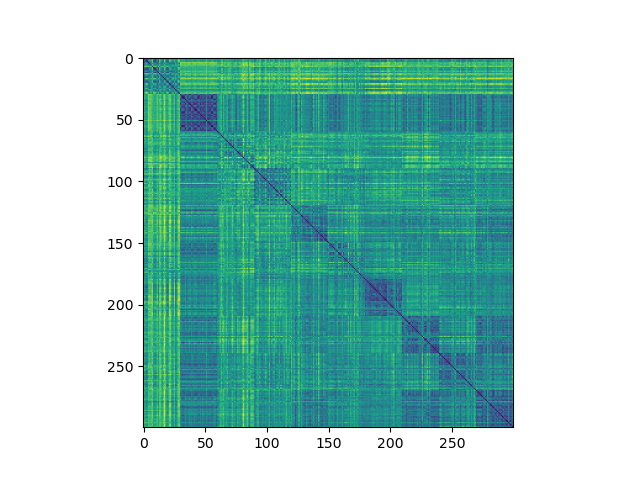
\includegraphics{l2_similarity_matrix.png}

We then found the image-wise differences using our method. When using
our model to find the image similarity between image A and image B, we
pass the images into the model in both orders, first mapping image A to
B then vice versa. We then take the maximum image difference found as
the final difference between the images. This image similarity matrix
kept the low distances between images of ``1''s, but also made many
other digits more similar to each other. This is likely because our
model corrected any small handwriting differences between images to
better align images with semantically similar content.

One finding to note is that the ``0'' and ``1'' digits were found to be
the most different from each other, which is consistent with human
perception of the digits. Overall, the difference matrix values were
lower than that of the \(L_2\) distance metric because our model acts as
a pseudo-\(L_2\) difference, but optimizes the pixel placement to
minimize the image difference. It is only possible for our model to
achieve approximately the same or lower values in the similarity matrix
as the baseline \(L_2\) distance method since an image where no pixels
are shifted (the \(L_2\) difference) is within the feasible set of our
model.

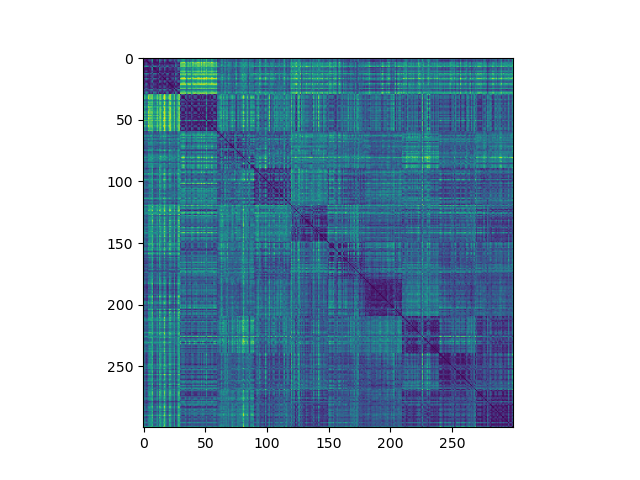
\includegraphics{optimization_similarity_matrix.png}

To confirm the optimization model works as intended, we translate a
single digit image by one pixel in all directions and map it to the
original image. Since the images of the MNIST dataset have some
background padding, each image should be able to map to the original
without difficulty (having all pixels moving in the same direction
except for some border pixels). In the example below, we display the
pixel movement of pixels with value greater than 0 (not part of the
background) at the various translations. We observe that the pixel
displacement correctly aligns the displaced images with the original.
Also, the image without displacement correctly does not shift any
pixels.

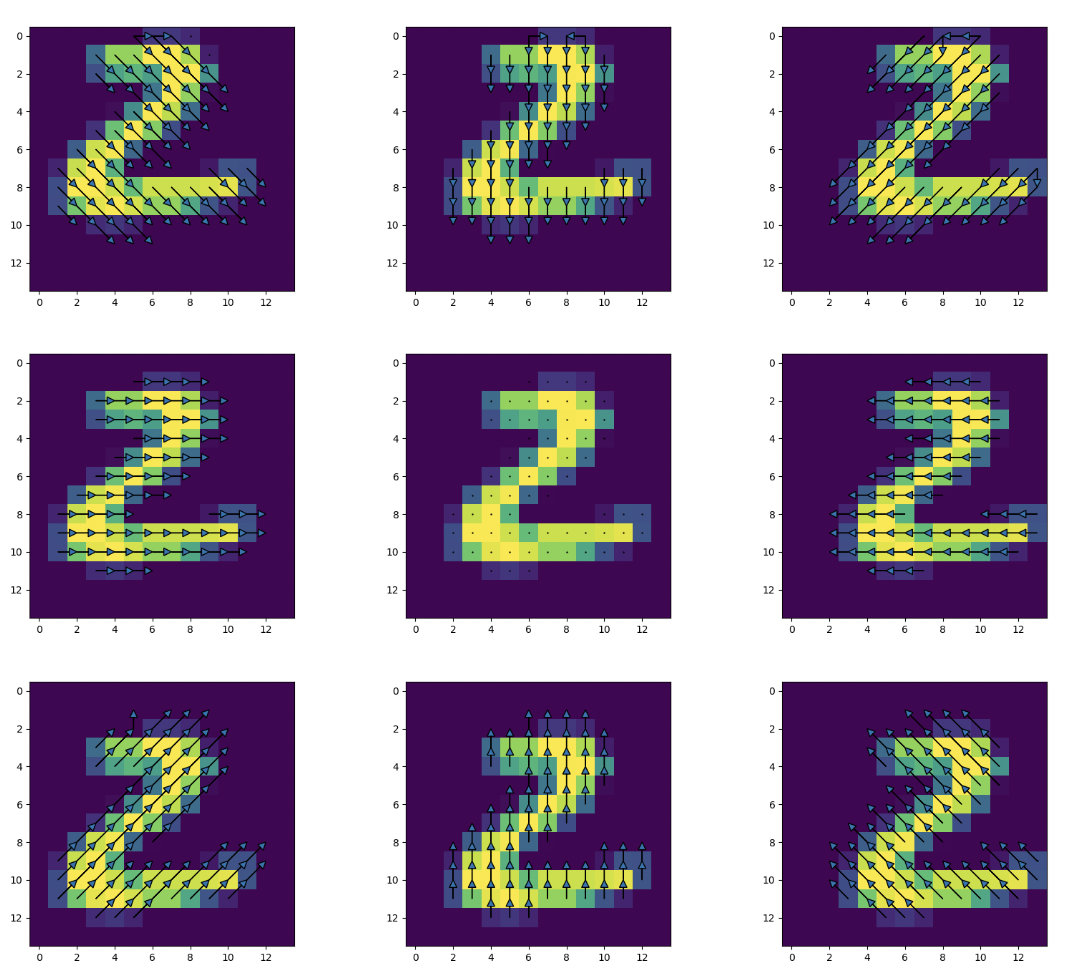
\includegraphics{example_2_shift.png}

One limitation of our approach is scalability. We had to confine the
possible window where each pixel could shift to the 9x9 area directly
around the starting location. We also had to downsize the MNIST images
to 14x14 to ensure the runtime of our algorithm was less than 1 min per
distance calculation. In practice, it is expected that pixel content
will shift more than 1 pixel in any direction and that the images being
compared will be much higher resolution (1000's of pixels)

An assumption that our approach makes is that pixels do not criss-cross.
However, this assumption only holds if images are similarly oriented.
When comparing the distance between two images which are mirrored or
rotated, our model will not work as intended because the pixels are not
allowed to change their relative positioning with respect to the x and y
axes. Considering a horizontally flipped image, it is clear that the
optimal repositioning of pixels should be to cross all pixels with
respect to the x axis.

    \hypertarget{b.-image-transformation}{%
\subsubsection{4.B. Image
Transformation}\label{b.-image-transformation}}

    We further tested our algorithm on image transformation with synthetic
data showing transformations such as scaling. Our method can be used as
an optimization-based method to compute pixel velocities in videos. We
compare our algorithm with the commonly-used pixel-tracking algorithm,
Optical Flow. We show test cases below of the output of the pixel
movement necessary to achieve the Target Object Size. Our algorithm
performs similar to optical flow for this synthetic data. Although, we
note that optical flow does not map to all pixels in the destination
image while our method does.

\begin{longtable}[]{@{}
  >{\centering\arraybackslash}p{(\columnwidth - 4\tabcolsep) * \real{0.3333}}
  >{\centering\arraybackslash}p{(\columnwidth - 4\tabcolsep) * \real{0.3333}}
  >{\centering\arraybackslash}p{(\columnwidth - 4\tabcolsep) * \real{0.3333}}@{}}
\toprule\noalign{}
\begin{minipage}[b]{\linewidth}\centering
Target Size 1
\end{minipage} & \begin{minipage}[b]{\linewidth}\centering
Our Method
\end{minipage} & \begin{minipage}[b]{\linewidth}\centering
Optical Flow
\end{minipage} \\
\midrule\noalign{}
\endhead
\bottomrule\noalign{}
\endlastfoot
& & \\
\end{longtable}

\begin{longtable}[]{@{}
  >{\centering\arraybackslash}p{(\columnwidth - 4\tabcolsep) * \real{0.3333}}
  >{\centering\arraybackslash}p{(\columnwidth - 4\tabcolsep) * \real{0.3333}}
  >{\centering\arraybackslash}p{(\columnwidth - 4\tabcolsep) * \real{0.3333}}@{}}
\toprule\noalign{}
\begin{minipage}[b]{\linewidth}\centering
Target Size 2
\end{minipage} & \begin{minipage}[b]{\linewidth}\centering
Our Method
\end{minipage} & \begin{minipage}[b]{\linewidth}\centering
Optical Flow
\end{minipage} \\
\midrule\noalign{}
\endhead
\bottomrule\noalign{}
\endlastfoot
& & \\
\end{longtable}

    These test cases show how the pixels in the source image need to move in
order to transform to the target image. An arrow for each pixel
determines how that pixel in the source image should move in order to
attain the target image. No Arrow means no movement is necessary. One
peculiarity of our method is that a single pixel can spread itself
across its neighboring region. As can be seen in the middle column,
certain pixels map into two or three different neighboring locations,
expanding the pixel. In contrast, optical flow relies on the assumption
that a pixel in the source image will be found (along with its
neighbors) in one location in the subsequent image. This requirement
limits optical flow to consider a one-to-one mapping whereas our method
is more flexible and supports one-to-many pixel mappings. Like Optical
Flow, our method determines the magnitude and direction of pixel
movement, thus allowing velocity computation on dynamic scenes. Our
method can be used as a replacement to optical flow. Currently, our
method is not nearly as performant, as optical flow can run at real-time
speeds (\textgreater30 FPS) on larger images.

    \hypertarget{conclusion}{%
\subsection{5. Conclusion}\label{conclusion}}

We have proposed a novel Mixed Integer Programming Optimization-based
image distance metric. Our method successfully showed how it can align
similar looking images in order to aid with image similarity metrics and
optical flow computation. First, our digit similarity matrix shows a
proof of concept that this method can be used to improve digit
classification if a user was to use k-nearest-neighbor classification.
Second, our method can compute pixel-level movement between subsequent
images which makes it a candidate replacement to the commonly-used
optical flow algorithm. Lastly, this method of image alignment has
applications as a general image distance between various images which
involve non-global stretching/expanding of the image. Another example
use case is image registration for biomedical images, since tissue
samples are commonly stretched between sample images, but maintain the
global positioning of features relative to each other.

Moving forward we would like to expand our method by making the model
more efficient and scalable. Our runtime seems to increase exponentially
with respect to the image and search window sizes, making it infeasible
for high resolution images. We would also like to consider how our
method could be modified to handle cases involving image
flipping/rotation. One potential idea comes from Scale-Invariant Feature
Transform (SIFT) features, in which the orientation of the image would
first be calculated, and then the pixel shifts would be constrained with
respect to the orientation of the image instead of the x and y axes.

    \begin{tcolorbox}[breakable, size=fbox, boxrule=1pt, pad at break*=1mm,colback=cellbackground, colframe=cellborder]
\prompt{In}{incolor}{ }{\boxspacing}
\begin{Verbatim}[commandchars=\\\{\}]

\end{Verbatim}
\end{tcolorbox}


    % Add a bibliography block to the postdoc
    
    
    
\end{document}
